%Modelo para escrita de artigos científicos do Trabalho de Conclusão de Curso da Engenharia de computação
% Unoesc - Campus de Joaçaba

%Se você é novo no latex, um bom lugar para começar é
%https://pt.overleaf.com/learn

\documentclass[10pt,conference,twocolumn]{unoesc} 

% -------------------- Configuração para usar trecho de código --------------------

\usepackage[utf8]{inputenc}
\usepackage[T1]{fontenc}
\usepackage{listings}
\usepackage{xcolor}

\lstset{
    language=C++,
    basicstyle=\scriptsize\ttfamily, % Reduzido de \footnotesize para \scriptsize
    keywordstyle=\bfseries,
    stringstyle=\itshape,
    commentstyle=\slshape,
    numbers=left,
    numberstyle=\scriptsize, % Ajustado de \tiny para \scriptsize
    stepnumber=1,
    numbersep=8pt, % Aumentado de 5pt para 8pt
    showspaces=false,
    showstringspaces=false,
    frame=single,
    breaklines=true,
    breakatwhitespace=true,
    tabsize=2,
    xleftmargin=14pt, % Nova margem à esquerda para afastar o código da borda
    xrightmargin=5pt, % Nova margem à direita para balancear
    aboveskip=0.5em, % Reduz espaço acima do código
    belowskip=0.5em, % Reduz espaço abaixo do código
    literate={á}{{\'a}}1 {é}{{\'e}}1 {í}{{\'i}}1 {ó}{{\'o}}1 {ú}{{\'u}}1
             {ã}{{\~a}}1 {õ}{{\~o}}1 {â}{{\^a}}1 {ê}{{\^e}}1 {ô}{{\^o}}1
             {ç}{{\c{c}}}1 {à}{{\`a}}1,
}

% ---------------------------------------------------------------------------------

\usepackage{csquotes}
%Use esse arquivo para incluir novos pacotes

\usepackage[%usado para determinar medidas
top=1.78cm,
bottom=1.78cm,
left=1.65cm,
right=1.65cm,
headsep=0cm,
%showframe
]{geometry}
%\usepackage[justification=centering]{caption}
\usepackage{times}
\usepackage{enumitem}%redefinir espacos itemize
\usepackage{graphicx}
\usepackage{url,hyperref}
\usepackage[utf8]{inputenc}
\usepackage{float}%mais controle para manipular figuras
\usepackage{caption}%manipular legenda da figura e tabela
\usepackage{mathtools}%equacoes
\usepackage[hang,flushmargin]{footmisc} 
\usepackage{xcolor}
\usepackage{wrapfig} %usado para envolver figura com texto
%\usepackage[portuguese]{babel}
\usepackage{fancyhdr}%criacao do cabecalho
\usepackage{etoolbox}
\usepackage[export]{adjustbox}%mais controle para ajustar tamanho da tabela
\usepackage{comment}%ambiente para comentario
\usepackage{relsize} %usado por comandos \mathlarger
\usepackage{lipsum} 

%Referencia bibliografica
\usepackage[
    style=numeric,
    sorting=none,
    maxbibnames=10]{biblatex}
\addbibresource{referencia.bib}

%Idioma. Use "english" para trabalhos em inglês
\usepackage[brazil]{babel}
%Ajustes na legenda da figura. Incluindo espacamento apos a legenda
\captionsetup[figure]{labelformat={default},labelsep=period,font=footnotesize, name=\footnotesize{Fig.},justification=centering,singlelinecheck=false,belowskip=0\normalbaselineskip}
%\pagenumbering{gobble}

%Ajustes na legenda da tabela. 
\captionsetup[table]{labelformat={default},labelsep=newline,font={sc,footnotesize},justification=centering,singlelinecheck=false}

%\renewcommand{\headrulewidth}{0pt}

% Renomear a legenda de listings para Português sem usar caption (evita conflitos)
% Para o pacote `listings` (ambiente `lstlisting`)
\renewcommand{\lstlistingname}{Código}
% Renomear também o título da lista de listings, se usado
\renewcommand{\lstlistlistingname}{Lista de Códigos}

\makeatletter
\newcommand{\linebreakand}{%
  \baselineskip 
  \end{@IEEEauthorhalign}
  \hfill\mbox{}\par
  \mbox{}\hfill\begin{@IEEEauthorhalign}
}
\makeatother


%%%%%%%%%%%%%%%%%%%%%%%%%%%%%%%%%%%%%%%%%%%%%%%%%%%%%%%%%%%%%%%%%%%%%%%%%
%    Configuracaoes de Idioma
%    Considerando babel = brazil
%%%%%%%%%%%%%%%%%%%%%%%%%%%%%%%%%%%%%%%%%%%%%%%%%%%%%%%%%%%%%%%%%%%%%%%%% 

\addto\captionsbrazil{
  \renewcommand{\abstractname}{Abstract}
  \renewcommand{\tablename}{TABELA}
}

%considerando babel = english
\addto\captionsenglish{
  \renewcommand{\tablename}{TABLE}
}

\begin{document}


  \title{Interface Gráfica Integrada ao ROS para Telemetria e Parametrização de Robô Autônomo}
  \author
  {
    \IEEEauthorblockN{Rafael Corrêa Zart\\}
    \IEEEauthorblockN{Orientador: Kleyton Hoffmann\\}
    \IEEEauthorblockA{Universidade do Oeste de Santa Catarina - Unoesc\\
                    ACET - Área de Ciências Exatas e Tecnológicas \\
                    Curso de Engenharia de Computação - 
                    Campus de Joaçaba/SC}
  }

\maketitle

 \vspace{0.3cm}
  \begin{resumo}
     %%%%%%%%%%%%%% Não retirar este trecho
    \noindent\footnote{Trabalho de Conclusão de Curso apresentado ao Curso de Engenharia de Computação no segundo semestre de 2025, Área de Ciências Exatas e Tecnológicas da Universidade do Oeste de Santa Catarina como requisito parcial à obtenção do grau de bacharel em Engenharia de Computação.}
     %%%%%%%%%%%%%% Não retirar este trecho
     Este trabalho propõe o desenvolvimento de uma interface gráfica para telemetria e parametrização de robôs autônomos, integrada ao \textit{Robot Operating System} (ROS) por meio do protocolo ROSBridge. Utilizando a biblioteca Streamlit, a interface foi projetada para oferecer interação intuitiva, com visualização em tempo real de velocidade, posição e mapas 2D gerados por algoritmos SLAM (\textit{Simultaneous Localization and Mapping}), além de possibilitar ajustes de parâmetros operacionais e controle manual do robô. A metodologia empregada estrutura-se em três fases distintas: a caracterização do \textit{hardware}, o desenvolvimento modular e a validação em ambientes simulados (RViz) e reais. O desenvolvimento modular encontra-se concluído, com o módulo de visualização e de controle implementados. \textit{Scripts} de comunicação via ROSBridge estão operacionais e integrados à interface e funcionalidades como o mapeamento 2D com LiDAR (Light Detection and Ranging) e a implementação de \textit{waypoints} estão funcionando. Funcionalidades planejadas na primeira fase de desenvolvimento do trabalho de conclusão de curso, como plotar mapa 2D com nuvem de pontos e navegação autônoma por waypoints foram implementadas com sucesso, testes também foram realizados para validar a precisão de posicionamento no mapa e a eficácia da interface. O sistema demonstra potencial para aplicações em ambientes internos e semi-estruturados, contribuindo para a integração eficiente entre interfaces gráficas e sistemas robóticos.
     
  \end{resumo}
  
  \begin{palavraschave}
    aplicativo, app, interface gráfica, LiDAR, robô autônomo, ROSBridge, Streamlit, web.
  \end{palavraschave}
  
  \vspace{0.5cm}
  
  \begin{abstract}
  \noindent This work proposes the development of a graphical interface for telemetry and parameterization of autonomous robots, integrated with the \textit{Robot Operating System} (ROS) through the ROSBridge protocol. Using the Streamlit library, the interface was designed to offer intuitive interaction, with real-time visualization of velocity, position, and 2D maps generated by SLAM (\textit{Simultaneous Localization and Mapping}) algorithms, in addition to enabling adjustments of operational parameters and manual control of the robot. The methodology employed is structured in three distinct phases: \textit{hardware} characterization, modular development, and validation in simulated (RViz) and real environments. The modular development is concluded, with the visualization and control modules implemented. \textit{Scripts} for communication via ROSBridge are operational and integrated into the interface, and functionalities such as 2D mapping with LiDAR and the implementation of \textit{waypoints} are working. Planned features for the first development phase of the undergraduate thesis, such as plotting 2D maps with point clouds and autonomous navigation by waypoints were implemented successfully, tests were also conducted to validate the positioning accuracy on the map and the interface's effectiveness. The system demonstrates potential for applications in indoor and semi-structured environments, contributing to the efficient integration between graphical interfaces and robotic systems.
  \end{abstract}

  \begin{IEEEkeywords}
    application, app, Autonomous robot, graphical interface, LiDAR, ROSBridge, Streamlit, web.
  \end{IEEEkeywords}
  
    \vspace{0.5cm}
\section{Introdução}

% A introdução deve conter uma visão geral sobre o tema, uma explicação geral do que o trabalho pretende com ou sem suporte de trabalhos correlatos. Nesta seção também deve estar clara a descrição do problema, a justificativa, os objetivos e a organização do trabalho.

% ----------------------------------- Contextualização do Tema -----------------------------------

A robótica autônoma tem se tornado cada vez mais presente em aplicações críticas que abrangem desde operações em ambientes extremos até tarefas cotidianas de automação. Estudos recentes na área destacam que a eficácia operacional desses sistemas depende fundamentalmente da integração harmoniosa entre interfaces de usuário bem projetadas e arquiteturas de controle confiáveis. Essa combinação estratégica não apenas possibilita uma interação mais intuitiva entre humanos e máquinas, mas também garante a execução autônoma eficiente de missões complexas, mantendo sempre a capacidade de supervisão e intervenção humana quando necessária \cite{IntroAR}.
 
% --------------------------------

Eu gosto de estudar robótica autônoma, e tenho interesse em desenvolver uma interface gráfica para controle de robôs autônomos, integrando-a com o ROS (Robot Operating System) para facilitar a comunicação e o controle em tempo real. O objetivo é criar uma plataforma que permita a visualização de dados sensoriais, a definição de metas de navegação e o controle manual do robô, utilizando tecnologias modernas de desenvolvimento de interfaces. A motivação para este projeto surge da necessidade de melhorar a interação entre humanos e robôs, tornando o controle mais acessível e eficiente, especialmente em ambientes internos onde a navegação autônoma pode ser desafiadora \cite{IntroROS}.

% -------------------------------- Estado da Arte / Revisão Breve --------------------------------

Estudos na área de robótica autônoma demonstram que os sistemas de controle para essas plataformas normalmente empregam técnicas consolidadas como controladores PID (proporcional integral derivativo), lógica \textit{fuzzy} e redes neurais \cite{KleytinhoBasico}. No âmbito das interfaces gráficas, observa-se uma diversidade de abordagens, desde soluções \textit{desktop} baseadas em ROS até interfaces \textit{mobile} para Android, cada uma com seus requisitos específicos de integração \cite{robo2wd, Teleoperacao}. Um desafio comum identificado na literatura é a dificuldade em estabelecer uma comunicação eficiente entre o núcleo de controle do robô e diferentes tipos de interfaces gráficas, frequentemente resultando em atrasos indesejados ou perda de sincronismo nos dados, independentemente da plataforma utilizada \cite{IntroROS}.

% ------------------------------------- Problema de Pesquisa -------------------------------------

A integração entre interfaces gráficas e sistemas de controle representa um dos principais desafios na robótica autônoma, impactando diretamente a eficácia operacional das plataformas robóticas \cite{IntroAR, IntroROS}. Este trabalho propõe uma solução que combina interfaces intuitivas com algoritmos de controle adaptativos, atendendo aos requisitos críticos de usabilidade e desempenho em sistemas robóticos autônomos.

% ---------------------------------------- Justificativa -----------------------------------------

A relevância desta pesquisa se manifesta em três aspectos principais: a otimização da interação humano-robô, essencial para sistemas de controle e supervisão; a contribuição para arquiteturas padronizadas, facilitando a replicabilidade de soluções; e a aplicação em cenários complexos, como navegação em ambientes dinâmicos e inspeção automatizada \cite{IntroROS}.

% ------------------------------------------ Trekking --------------------------------------------

A modalidade \textit{Trekking} em competições robóticas desafia os robôs a navegarem autonomamente em terrenos irregulares, superando obstáculos utilizando fusão de dados sensoriais (LIDAR, IMU e câmeras) para mapeamento 3D e tomada de decisão \cite{KleytinhoBasico}. As regras avaliam não apenas a conclusão do percurso, mas também critérios como suavidade de movimento, eficiência energética e precisão de posicionamento (tolerâncias $\leq$ 5~cm). Essas regras tornam o ambiente de competição um \textit{benchmark} ideal para validar sistemas robóticos integrados, já que exige interfaces gráficas responsivas, algoritmos de controle adaptativos e comunicação robusta, requisitos que demonstram transferibilidade direta para aplicações práticas como agricultura de precisão e inspeção de infraestruturas \cite{KleytinhoBasico}.

% ------------------------------------------ Objetivos -------------------------------------------

O objetivo central do meu trabalho consiste no desenvolvimento de uma plataforma robótica integrada, com dois focos específicos: implementação de uma interface gráfica otimizada para controle robótico e validação em ambientes característicos de aplicações robóticas \cite{IntroAR, IntroROS}.

% ------------------------------------- Metodologia (Breve) --------------------------------------

Partindo da plataforma robótica já adquirida para o projeto, o desenvolvimento seguirá uma abordagem prática em três etapas integradas. Na fase inicial, será realizada a caracterização detalhada do \textit{hardware} disponível, mapeando suas capacidades e limitações para orientar o projeto da interface gráfica e dos algoritmos de controle. A implementação adotará uma arquitetura modular, com desenvolvimento paralelo e teste individual de cada subsistema (interface móvel, núcleo de controle e módulo de comunicação) seguindo padrões de interoperabilidade consagrados na área. A etapa final consistirá na integração progressiva e validação do sistema completo, com testes em condições reais de operação que aproveitem plenamente as capacidades da plataforma física disponível, assegurando robustez e desempenho adequados às aplicações planejadas.

% ------------------------------------- Estrutura do Artigo --------------------------------------

Este artigo está estruturado em sete seções. Na seção I, foi introduzido o tema da robótica autônoma e os desafios na integração interface-controle, com os objetivos do trabalho. Na seção II, foram abordados os conceitos teóricos fundamentais sobre navegação autônoma, algoritmos de controle e protocolos de comunicação. Na seção III, foram examinadas pesquisas anteriores sobre sistemas similares, identificando lacunas a serem superadas e ideias a serem exploradas. Na seção IV, foi descrita a metodologia em três fases: caracterização do hardware, desenvolvimento modular e validação. Na seção V, foram mostrados os resultados dos testes de desempenho do sistema. Na seção VI, foram apresentados os resultados finais em condições reais de operação. Na seção VII, foram destacadas as conclusões e sugestões para trabalhos futuros.
\section{Referencial Teórico}
\label{sec:referencial}

Neste capítulo são apresentadas as tecnologias: robótica autônoma, telemetria, mapeamento, planejamento de trajetória e API, que foram utilizadas para o desenvolvimento do trabalho, com o objetivo de familiarizar o leitor a ter uma leitura mais compreensiva do mesmo.


\subsection{Robótica Autônoma}
A robótica autônoma tem evoluído continuamente, tornando-se cada vez mais relevante no cenário tecnológico atual. A capacidade dos robôs autônomos substituírem humanos em atividades perigosas ou repetitivas justifica os investimentos na área. Competições e projetos educacionais desempenham papel fundamental na formação de profissionais e no estímulo ao interesse pela robótica \cite{RoboAutonomo}.

Alguns dos principais desafios são navegação, planejamento de trajetória, localização e desvio de obstáculos \cite{AMRChallenges}. Os sistemas de navegação de robôs móveis dependem do nível de abstração da representação do ambiente \cite{Mapeamento}. Para determinar com precisão a posição e a orientação do robô móvel, é essencial que o ambiente seja modelado em uma estrutura simples e compreensível.
A parte desafiadora da localização é estimar a posição do robô e a orientação da qual essa informação pode ser obtida de sensores e outros sistemas. Para lidar com o desafio da localização, uma boa técnica deve ser desenvolvida para tratar erros, fatores de interferência, medições incorretas e estimativas imprecisas \cite{Odometria}. Desvio de obstáculos é uma tarefa essencial no campo da robótica, pois é fundamental que o robô alcance seu destino sem ser bloqueado por qualquer obstáculo ou sofrer colisões em seu trajeto \cite{PlanejamentoTrajetoria}. Por esse motivo, algoritmos livres de colisão são um requisito indispensável para robôs móveis autônomos \cite{IntroAR, AMRChallenges}.

Os robôs autônomos têm aplicações variadas: podem atuar desde o campo, monitorando lavouras, até ambientes industriais, seja atuando em processos produtivos como linhas de montagem e gestão logística de estoques em armazéns.

\subsection{ROS}
O Robot Operating System (ROS) é um conjunto de bibliotecas de \textit{software} e ferramentas que auxiliam no desenvolvimento de aplicações robóticas. De \textit{drivers} a algoritmos de ponta, e com poderosas ferramentas para desenvolvedores, o ROS oferece o que você precisa para o seu próximo projeto de robótica. E tudo isso é de código aberto \cite{ROS_Website}.

O ROS vai além de ser apenas um conjunto de bibliotecas, ele funciona como um ecossistema robusto que padroniza a comunicação entre diferentes componentes de software em um robô. Ele oferece um modelo de programação distribuída, onde múltiplos nós (programas executáveis independentes) podem se comunicar enviando e recebendo mensagens através de tópicos. Isso permite que desenvolvedores de diversas áreas colaborem em um mesmo projeto robótico, com cada um focando em um módulo específico (como navegação, percepção ou controle), e o ROS garantindo a integração.

\subsection{Telemetria}
A palavra telemetria é a união de duas palavras gregas. \textit{Tele} significa longe e 
\textit{meter} significa medir. Por isso, telemetria significa realizar medições à distância, ou em local remoto. Os ingredientes essenciais de qualquer sistema de telemetria incluem pelo menos um sensor, uma antena transmissora de baixo ganho, uma antena receptora de alto ganho, um receptor e um mostrador \cite{Telemetria}. 

Teste de veículos foi uma das primeiras aplicações da telemetria. Inicialmente, não tripulados, como mísseis guiados, requeriam telemetria, para que os engenheiros soubessem o que se passava dentro do míssil. Veículos tripulados também requeriam telemetria para medir parâmetros, tais como fadiga da asa, que não eram perceptíveis aos tripulantes 
\cite{Telemetria}.

\subsection{Mapeamento e Planejamento de Trajetória}
A técnica geral de \textit{roadmap} para planejamento de trajetórias consiste em capturar a conectividade do espaço livre do ambiente em uma rede de curvas de uma dimensão, denominada \textit{roadmap}. Uma vez que esta rede tenha sido obtida, ela é vista como um conjunto padrão de caminhos. O planejamento de trajetórias reduz-se então a conectar as posições iniciais e finais do robô ao \textit{roadmap} e buscar neste um caminho entre esses dois pontos, conforme pode ser observado na Figura \ref{fig:roadmap} \cite{PlanejamentoTrajetoria}.

\begin{figure}[h]
    \centering
    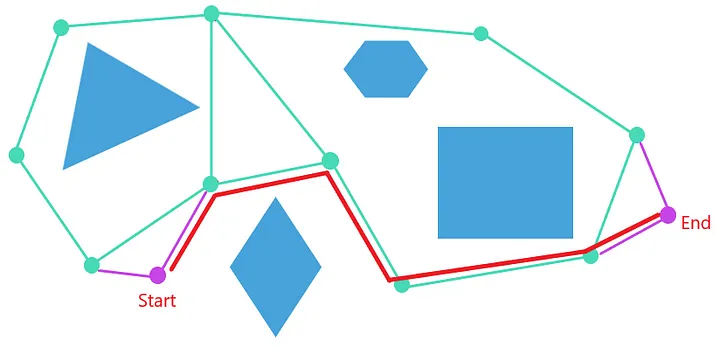
\includegraphics[width=0.45\textwidth]{images/RoadmapRT.png}
    \caption{Gráfico de navegação \textit{roadmap} para encontrar a melhor rota.}
    \label{fig:roadmap}
    % Referência: https://arushi-khokhar.medium.com/probabilistic-roadmap-prm-for-path-planning-in-robotics-d4f4b69475ea
\end{figure}

Quando não há um mapa do ambiente obtido a \textit{priori}, é preciso construir o mapa durante a navegação. Nesse caso, técnicas de localização e mapeamento simultâneo (SLAM) são usadas \cite{SLAM}.

Resolver o problema de SLAM envolve a estimação da trajetória do robô e do mapa do ambiente enquanto o robô se desloca. Ao longo da movimentação do robô em poses sequenciais desconhecidas \( x_{1:t} = x_1, x_2, \ldots, x_t \) em um mapa desconhecido \( m \), são obtidas uma sequência de odometria \( u_{1:t} = u_1, u_2, \ldots, u_t \) e observações do ambiente \( z_{1:t} = z_1, z_2, \ldots, z_t \). O problema SLAM requer a obtenção da distribuição de probabilidades dada pela Equação 1, considerando que \( x_0 \) é a posição inicial do robô \cite{Mapeamento}.

O Cartographer é um sistema de SLAM eficiente que opera em dois níveis: localmente ajusta a pose do robô em submapas usando um \textit{scan matcher} (Ceres), enquanto globalmente refina a localização combinando todos os submapas em um mapa maior \cite{Cartographer, Ceres}. Sua principal vantagem é a flexibilidade, com suporte a múltiplos sensores e resoluções, e a eficiência computacional que permite operação em tempo real \cite{NVIDIA_JetsonOrinNano}.

Existe uma dificuldade intrínseca em conciliar as medições de localização com a posição verdadeira do dispositivo após longos períodos de navegação. O desafio origina-se na imprecisão dos sensores de medidas de odometria (ex: sonares, lasers e câmeras) devido às limitações físicas e imprevisibilidades do sistema \cite{Odometria}.

\subsection{API}
APIs (Interface de Programação de Aplicações) simplificam e aceleram o desenvolvimento de aplicativos e \textit{software}, permitindo que os desenvolvedores integrem dados, serviços e recursos de outros aplicativos, em vez de desenvolvê-los do zero. As APIs também oferecem aos proprietários de aplicativos uma maneira simples e segura de disponibilizar os dados e as funções dos aplicativos para os departamentos da organização. Os proprietários de aplicativos também podem compartilhar ou comercializar dados e funções para parceiros de negócios ou terceiros \cite{IbmAPI}.

As APIs permitem o compartilhamento apenas das informações necessárias, mantendo ocultos outros detalhes internos do sistema, o que auxilia na segurança do sistema. Os servidores ou dispositivos não precisam expor totalmente os dados: as APIs permitem o compartilhamento de pequenos pacotes de dados, relevantes para a solicitação específica \cite{IbmAPI}.

Podem existir vulnerabilidades de segurança devido à implementação da API. Por exemplo, a falha em verificar o tamanho dos \textit{inputs} na sua API pode permitir que um atacante derrube seu servidor ao enviar um \textit{input} extremamente grande que consuma toda a memória disponível - um tipo de ataque de negação de serviço (DoS) \cite{APISecurity}.

ROSBridge é uma especificação de protocolo de rede em camada de aplicação para o ROS (\textit{Robot Operating System}) que enfatiza o modelo cliente/servidor. Especificamente, o ROSBridge permite que clientes publiquem e escrevam mensagens em tópicos e invoquem serviços no ambiente de execução do servidor. O protocolo transporta mensagens formatadas em JSON por meio de \textit{sockets} TCP ou \textit{WebSockets} \cite{ROSBridge}.

No trecho de código \ref{lst:conexao_websocket} a classe roslibpy.ros é instanciada com o IP do dispositivo ROS e também a porta padrão para comunicação WebSocket, e o método client.run() inicia a conexão com o servidor ROS.   

\begin{lstlisting}[caption={Configuração da Conexão WebSocket com ROSBridge},label={lst:conexao_websocket}]
    import roslibpy
    
    # Configura a conexão WebSocket com o ROSBridge
    rosbridge_ws_url = '192.168.137.150'  # IP do dispositivo ROS
    client = roslibpy.Ros(host=rosbridge_ws_url, port=9090)

    # Conecta ao ROS
    client.run()
\end{lstlisting}
    
\subsection{Articulação das Tecnologias}
As tecnologias apresentadas neste referencial teórico articulam-se de forma coerente e complementar na solução desenvolvida. A robótica autônoma fornece a base conceitual para o sistema, enquanto as técnicas de telemetria e os protocolos de comunicação (ROSBridge) garantem a troca eficiente de dados entre os componentes. O SLAM e os algoritmos de planejamento de trajetória permitem a navegação autônoma, sendo acessíveis ao usuário através da interface desenvolvida com \textit{frameworks} modernos. As APIs, por sua vez, atuam como elemento integrador, possibilitando a comunicação segura entre a aplicação e o sistema robótico. Esta sinergia tecnológica resulta em uma plataforma completa que aborda desde a percepção ambiental até a interação com o usuário final, cumprindo os objetivos propostos de forma integrada e eficiente.
\section{Trabalhos Correlatos}
\label{sec:trabalhos}

% Sobre o que é, tecnologia utilizada, para que foi usado.
% O que faz?
% Por que é parecido?

Lima e Silva (2022) \cite{robo2wd} propuseram um sistema que viabiliza a programação e controle de um robô carro 2WD (duas rodas), utilizando Unity e C\# para desenvolver o aplicativo. O aplicativo tem as funções de ser servidor para múltiplos dispositivos e fornecer controle manual sobre um robô. Essa proposta se assemelha ao projeto do meu trabalho ao utilizar um aplicativo para o controle do robô autônomo.

Zago (2018) \cite{TelemetriaCompeticao} desenvolveu um sistema de telemetria sem fio para robôs de combate utilizando a tecnologia \textit{Bluetooth} para comunicação e o sistema operacional Android com um aplicativo para monitoramento do robô. O sistema de telemetria foi desenvolvido de uma maneira que não afeta diretamente  a funcionalidade, ou seja, o robô continua funcionando se o sistema de medição sofrer algum dano. Esse estudo se alinha a este trabalho pois utiliza a telemetria para comunicação com o robô e também utiliza um aplicativo para controle dos dados.

Werneck et al. \cite{TelemetriaSolar} elaboraram um sistema de telemetria para uma embarcação movida a energia solar para monitorar dados elétricos e de desempenho do barco solar em tempo real. Utilizaram um ESP32 para processamento, LoRa para transmissão de dados a longas distâncias, .NET para desenvolvimento da interface e outras tecnologias. O sistema mede e transmite dados para uma estação terrestre via LoRa ou conexão 4G. Os dados são processados e exibidos em uma interface gráfica desenvolvida em .NET para monitoramento e análise. Este projeto é semelhante ao meu estudo por utilizar tecnologias de telemetria e interface gráfica para monitoramento em tempo real de parâmetros do sistema embarcado.

Pico et al. \cite{Teleoperacao} propuseram um sistema de alarme e teleoperação em tempo real para falhas de navegação autônoma, comparando ROS 1 e ROS 2. O sistema integra uma interface web baseada em Vue.js e um \textit{joystick} com \textit{feedback} háptico para monitorar e controlar robôs em ambientes dinâmicos. A arquitetura utiliza sensores LiDAR (\textit{Light Detection and Ranging}), câmeras RGB-D e IMU para detectar colisões iminentes ou instabilidades em terrenos irregulares, acionando alertas visuais e vibrações no \textit{joystick}. Essa proposta se assemelha ao meu trabalho ao empregar uma interface gráfica para teleoperação e integração multimodal de sensores, com destaque para a comunicação via ROSBridge.

Perin et al. \cite{KleytinhoBasico} desenvolveram um robô móvel autônomo para competições ao ar livre, utilizando um chassi comercial adaptado. O sistema de percepção do robô é composto por um sensor de orientação de 9 eixos e um encoder incremental para localização e odometria. Para o controle de trajetória e velocidade, foram implementados controladores PID em C++, e o sistema foi simulado em um ambiente ROS integrado com a plataforma V-REP antes da implementação física. A proposta se assemelha ao meu trabalho ao empregar um sistema embarcado para o controle autônomo de um robô, com a particularidade de focar na navegação por coordenadas pré-definidas em campo aberto.
\section{Metodologia}
\label{sec:metodologia}

% ------------------------------- Apresentação Geral da Metodologia ------------------------------

Este trabalho adota uma abordagem metodológica estruturada em três fases para desenvolver uma interface gráfica intuitiva, estabelecer uma conexão robusta e validar o sistema em ambientes operacionais reais, com foco em robôs autônomos em ambientes internos e semi-estruturados. 

% --------------------------- Estratégia de Desenvolvimento e Validação --------------------------

A metodologia inicia com a análise do \textit{hardware} comercial disponível e a definição de requisitos técnicos. Em seguida, avança-se para o desenvolvimento paralelo dos subsistemas. Isso inclui a interface gráfica de usuário (GUI) com testes de usabilidade, a conexão robô-interface e os protocolos de comunicação via ROSBridge, conforme ilustrado na Figura \ref{fig:diagram}. O foco desta etapa é priorizar a exibição em tempo real de parâmetros essenciais, como posição, orientação e estado do sistema. Dessa forma, não são incorporados recursos avançados de aprendizado de máquina ou análise preditiva. A etapa final consiste em testes de integração e validação em ambientes simulados (RViz) e reais, limitados pelo período de desenvolvimento do trabalho acadêmico, o que restringe a quantidade de cenários avaliados.
% ---------------------- Abordagem Sequencial: Eficiência e Escalabilidade -----------------------

Essa abordagem sequencial assegura a verificação individual de cada componente antes da integração final, o que garante a eficiência operacional nas condições práticas previstas. Além disso, tal estrutura abre oportunidades para futuras expansões, como o desenvolvimento de componentes personalizados ou aplicações em ambientes externos.

\subsection{Análise do Hardware}
% -------------------------------- Caracterização do Hardware --------------------------------

A primeira fase da metodologia caracteriza o NVIDIA Jetson Orin Nano Developer Kit, plataforma do sistema robótico. O kit inclui um módulo Jetson Orin Nano 8GB com GPU NVIDIA Ampère (1024 núcleos CUDA), CPU de 6 núcleos e 8GB de memória LPDDR5, oferecendo até 40 TOPS (\textit{Tera Operations Per Second}) para aplicações de robótica. Sensores como LiDAR, IMU de 6 eixos e ultrassônicos, conectados via USB 3.2 Tipo-A ou conector de 40 pinos, suportam mapeamento 2D e navegação. Dois conectores MIPI CSI permitem câmeras para visão computacional. O armazenamento usa microSD ou SSD NVMe (M.2 Key-M). A comunicação ocorre via Wi-Fi, integrando com o ROS via ROSBridge \cite{NVIDIA_JetsonOrinNano}.


%Requisitos técnicos

%verificar 3D lidar ok

\subsection{Arquitetura do Sistema}

\begin{figure*}[htpb]
    \centering
    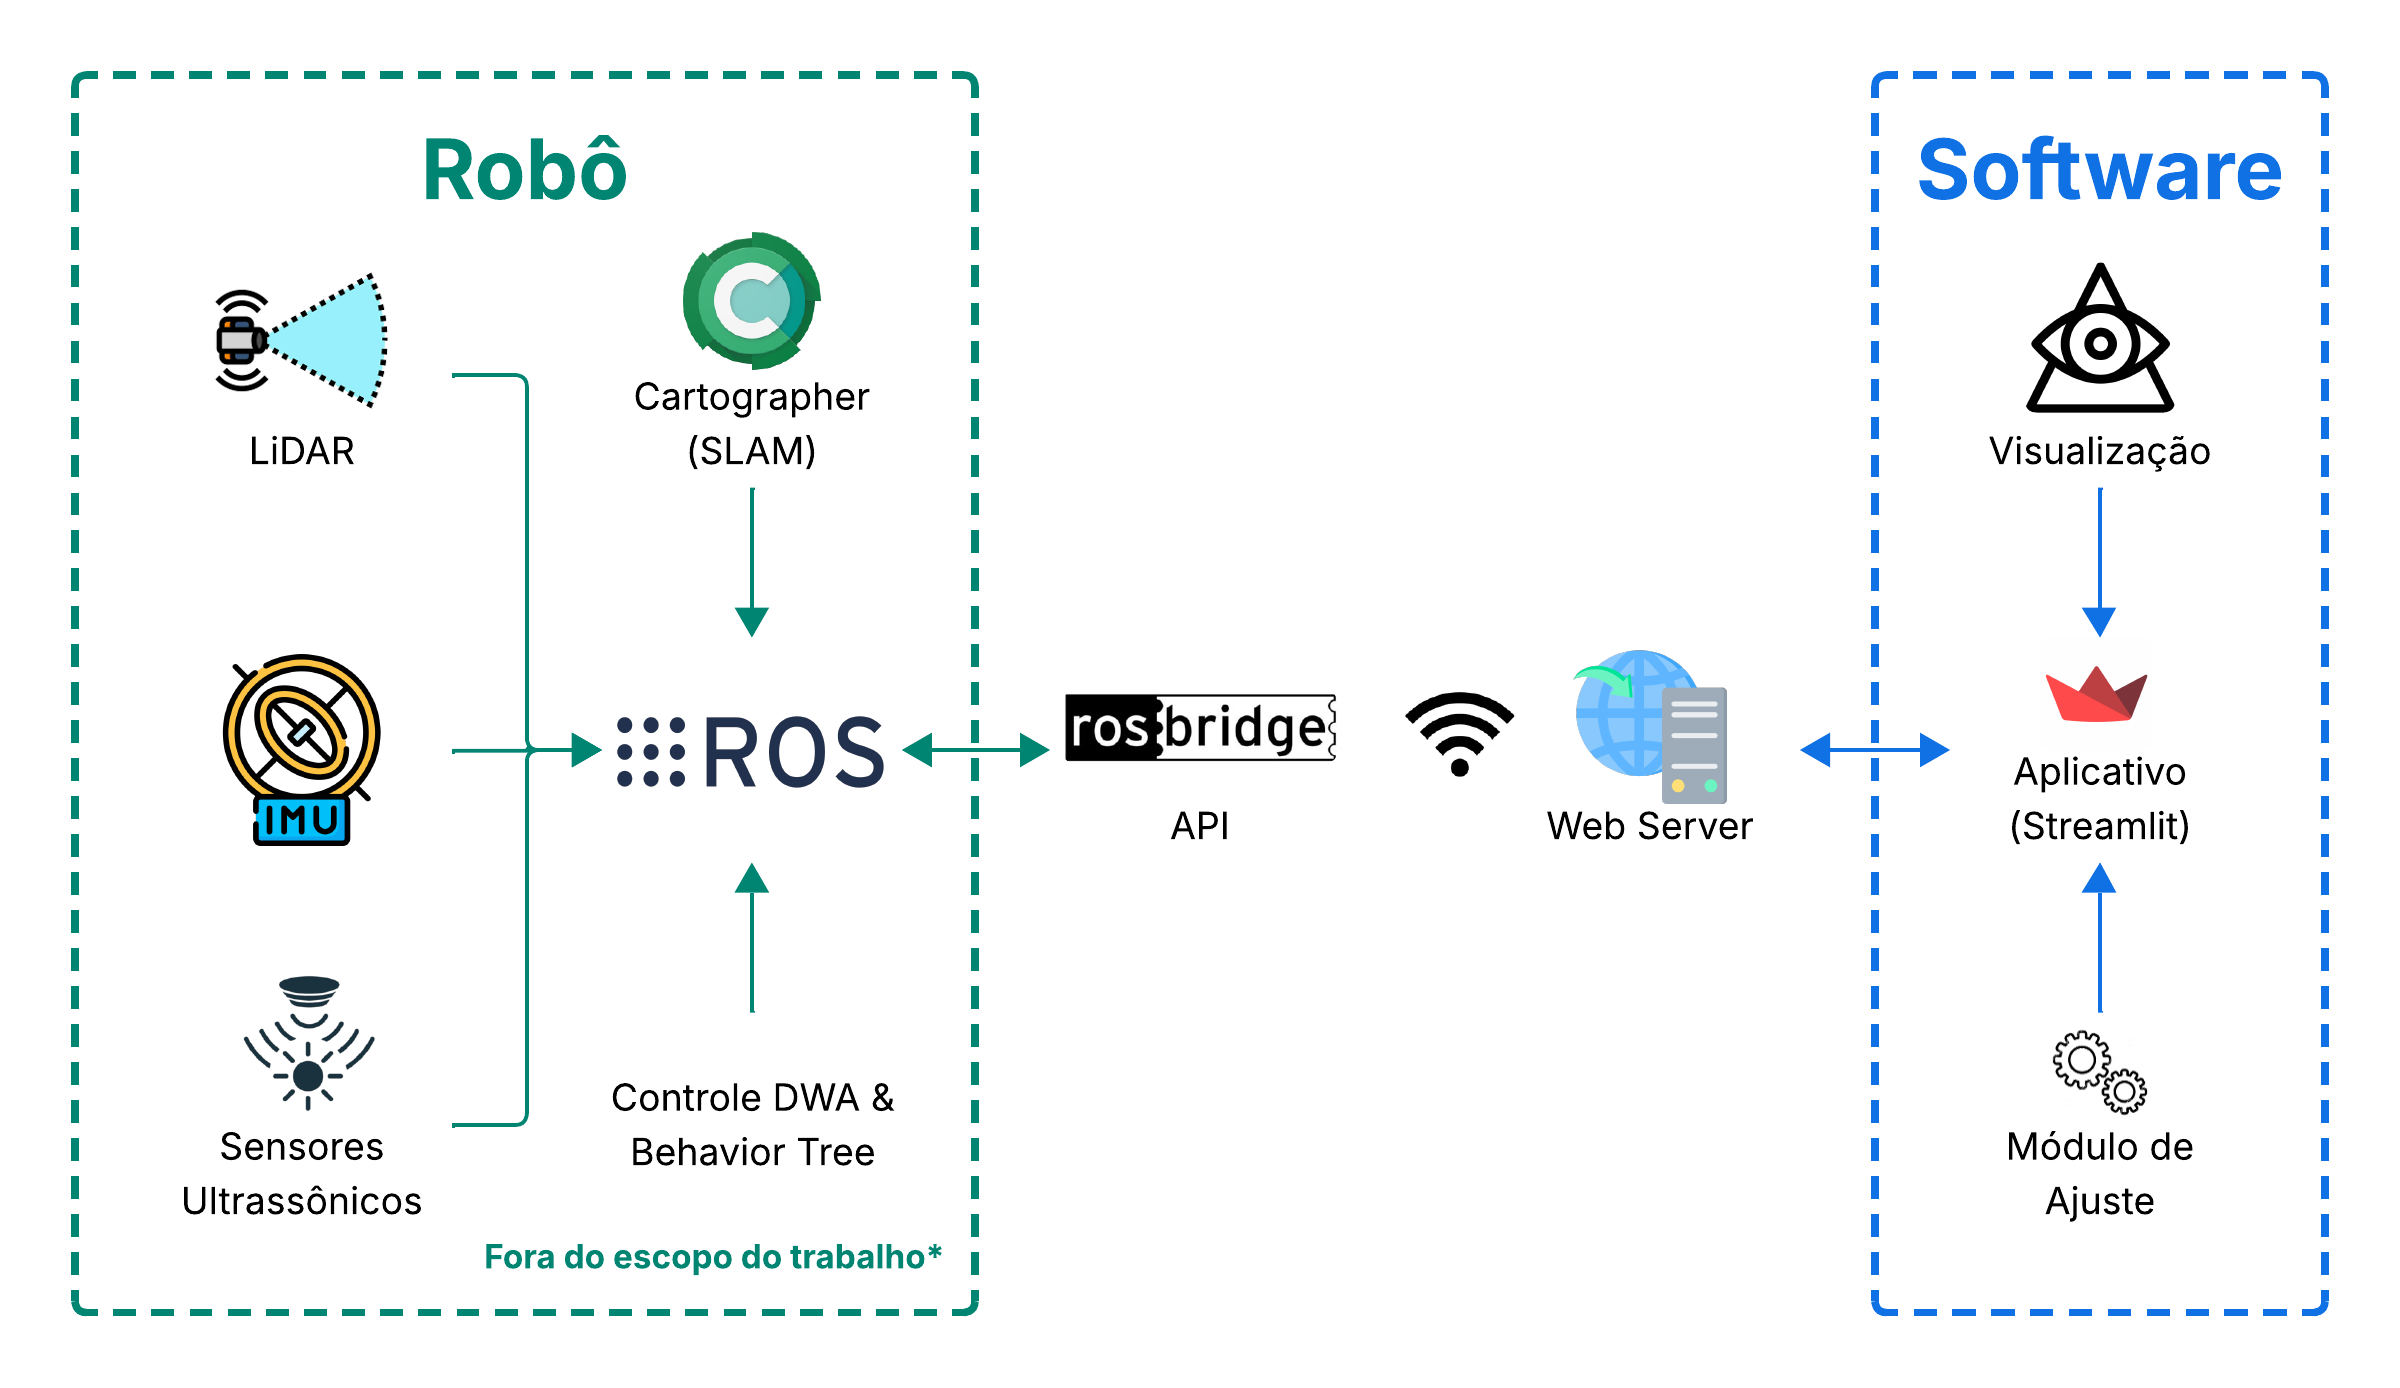
\includegraphics[width=\textwidth]{images/Diagrama_Arq.png}
    \caption{Diagrama da arquitetura do sistema.}
    \label{fig:diagram}
\end{figure*}

%fazer a chamada da figura no primeiro parágrafo. ok

O sistema robótico é projetado com uma arquitetura modular distribuída em três camadas principais, concebida para oferecer alta escalabilidade e flexibilidade na integração com diferentes plataformas robóticas e configurações de sensores. Na camada de percepção, os sensores atuam como os órgãos sensoriais do robô: um LiDAR para mapeamento 3D do ambiente, uma IMU de 6 eixos para medição inercial e sensores ultrassônicos para detecção de obstáculos próximos. 

A camada de processamento reside em um computador embarcado que opera o ROS (\textit{Robot Operating System}). Importante ressaltar que, apesar da nomenclatura, o ROS funciona como um \textit{framework} de software para robótica, e não como um sistema operacional em si. Essa camada estabelece a comunicação com os demais componentes através do ROSBridge, gerenciando a telemetria (incluindo dados de velocidade e status do sistema) e a integração direta com a interface. A ampla utilização do ROS como padrão na indústria e academia contribui para a facilidade de integração com uma diversidade de plataformas robóticas e dispositivos, o que intrinsecamente melhora a escalabilidade da arquitetura.

Na camada de interface com o usuário, o Streamlit \cite{Streamlit} fornece uma aplicação web acessível via navegador, exibindo dados de telemetria em tempo real e permitindo o controle manual quando necessário. A interface se conecta ao ROS através do ROSBridge, garantindo baixa latência na troca de comandos. Medidas de segurança como autenticação de usuário e criptografia serão implementadas para proteger a comunicação \cite{Streamlit}.

O fluxo de dados segue um ciclo contínuo: os sensores enviam informações para o ROS, que processa e toma decisões de navegação, enquanto a interface exibe os dados, recebe e envia comandos ao usuário. Os módulos são projetados para operar de forma independente em caso de falha pontual. A arquitetura desacoplada e a comunicação padronizada via ROS conferem ao sistema uma notável capacidade de adaptação e expansão, permitindo a integração com variados conjuntos de sensores e a fácil adição de novas funcionalidades.

% --------------------- Interface Gráfica ----------------------
%FAZER PROTÓTIPOS DE TELA E PENSAR NO FLUXO E USABILIDADE.
% VISUALIZAÇÃO PRÉVIA DE CADA MÓDULO
%CONTROLE
%VISUALIZAÇÃO DO MAPA - mapa, velocidade x, y, z, localização no mapa. Possibilidade de marcar pontos de passagem robo.
%Pensar como inserir lidar.
%CONFIGURAÇÃO/PARAMETRIZAÇÃO

%PARAMETRIZAÇÃO: velocidade mínima, velocidade máxima, modo teste, modo competição...

%https://balsamiq.com
O desenvolvimento da interface gráfica prioriza a criação de uma experiência intuitiva para o usuário final, com foco na implementação de um design responsivo que ofereça \textit{feedback} visual imediato para todas as interações. 

\begin{comment}
    
%não inserir nenhum parecer do que já foi feito na metodologia
A abordagem garantiu que a interface atendesse plenamente às necessidades de interação humano-robô, mantendo a simplicidade de uso sem comprometer a funcionalidade.
\end{comment}

% --------------------------- Comunicação ----------------------------

O módulo de comunicação é desenvolvido para garantir a troca de dados eficiente e confiável entre a interface e o robô. O protocolo ROSBridge é implementado para telemetria e integração com o sistema ROS, com atenção especial à redução de latência e manutenção da estabilidade da conexão.

%TROCAR TEMPO VERBAL DA METODOLOGIA - PRESENTE ok 

% ----------------------------- Tecnologias e Ferramentas Utilizadas -----------------------------

O sistema foi desenvolvido utilizando tecnologias complementares que atendem a cada componente específico. Para a interface, foi adotada a biblioteca Streamlit \cite{Streamlit}, que permite criar aplicativos web interativos com Python \cite{python3}, integrando-se diretamente ao núcleo do sistema ROS. Essa escolha elimina a necessidade de múltiplas linguagens e simplifica o desenvolvimento.

Também foram utilizadas outras duas bibliotecas Python: base64 para utilizar imagens no HTML e roslibpy\cite{ROSBridge} para comunicação da interface com o ROS.

A comunicação entre os módulos emprega o ROSBridge para telemetria geral e integração específica com o ROS. Essa combinação foi validada em trabalhos anteriores com requisitos semelhantes \cite{Teleoperacao}.

Para desenvolvimento e testes, o RViz\cite{rviz_wiki} está sendo utilizado para simulações iniciais e o Ceres Solver\cite{Ceres} para otimização numérica no mapeamento. A arquitetura resultante, apoiada por essas tecnologias validadas na literatura, oferece robustez operacional e facilidade de manutenção.

% -------------------------------- Requisitos da Interface --------------------------------

A interface gráfica para o sistema de telemetria e parametrização do robô autônomo é projetada com o objetivo de proporcionar uma interação intuitiva e eficiente entre o usuário e o robô, assegurando a visualização de dados em tempo real, a configuração de parâmetros operacionais e o controle manual, quando necessário. Com base na arquitetura modular e nas tecnologias empregadas, como o Streamlit e o protocolo ROSBridge, a interface é estruturada em dois módulos: Visualização e Controle. Esses módulos foram definidos para atender aos requisitos de usabilidade, alinhando-se aos objetivos do projeto e às demandas de interação humano-robô.

O módulo de visualização apresenta, em tempo real, informações essenciais como velocidade, posição e mapeamento do ambiente do robô. Esses dados são exibidos por meio de indicadores numéricos, com um mapa 2D gerado pelo algoritmo SLAM (Cartographer)\cite{Cartographer} para representar o terreno. Desenvolvida com Streamlit, a interface é responsiva, clara e acessível em dispositivos como navegadores web ou móveis, garantindo uma experiência amigável. A atualização dos dados ocorre com baixa latência, permitindo monitoramento contínuo.

O módulo de controle permite o usuário ajustar configurações operacionais, como limites de velocidade por meio de formulários interativos criados no Streamlit. Esses ajustes são enviados ao sistema via ROSBridge, garantindo uma comunicação rápida e segura. O módulo também oferece funcionalidades para operação manual utilizando setas direcionais para movimentação, essenciais em cenários que exigem intervenção humana, como testes ou situações de falha. A interface foi projetada para ser intuitiva, com elementos visuais que fornecem \textit{feedback} imediato, como confirmações de comandos. 

% ------------------------------ Critérios de Validação e Avaliação ------------------------------
\subsection{Critérios de Validação e Avaliação}

O sistema será avaliado em três aspectos principais: desempenho, robustez e usabilidade. 
 
% AVALIAR COMO SERÁ FEITO.

Os testes serão inicialmente realizados em ambiente simulado (RViz/ROS) para validação dos algoritmos e arquitetura. Após aprovação na simulação, o sistema será testado em condições reais, para verificar a robustez e a segurança da operação. Todos os resultados serão comparados com os requisitos técnicos estabelecidos.

% ------------------------------------- Limitações e Escopo --------------------------------------
\begin{comment}
%Mesclar esta informações no primeiro parágrafo da metodologia. De forma mais suave. ok


\subsection{Limitações e Escopo}

O presente trabalho foca no desenvolvimento de uma interface gráfica para telemetria e parametrização de robôs autônomos em ambientes internos e semi-estruturados, com algumas limitações definidas. Quanto ao escopo, não serão abordadas aplicações em ambientes externos ou condições climáticas adversas.

Quanto às limitações específicas da interface gráfica, o sistema está condicionado à visualização de dados provenientes exclusivamente dos sensores embarcados no robô, sem capacidade de fusão com fontes externas de informação ambiental. A arquitetura adotada prioriza a exibição de parâmetros essenciais para operação em tempo real, como posição, orientação e estado dos sistemas, em detrimento de visualizações 3D complexas ou reconstruções detalhadas do ambiente. A interface também não contempla recursos avançados de aprendizado de máquina para análise preditiva ou adaptação automática de layouts, mantendo-se focada em funcionalidades de telemetria e parametrização manual.

Em termos temporais, o projeto está limitado ao período de desenvolvimento do trabalho acadêmico, o que restringe a quantidade de cenários de teste que podem ser avaliados. Estruturalmente, a solução utiliza hardware comercial disponível, sem desenvolvimento de componentes eletrônicos customizados. Estas limitações, entretanto, abrem oportunidades claras para trabalhos futuros de expansão e aprimoramento do sistema.

\end{comment}
\section{Desenvolvimento}

A interface gráfica encontra-se concluída, tanto o componente visual (telas apresentadas na Seção \ref{sec:resultados}), quanto as funcionalidades como o mapa 2D gerado pelo LiDAR dentro do ROS e a implementação de \textit{waypoints} para navegação autônoma. As funcionalidades de controle estão operacionais.

A interface foi desenvolvida utilizando a biblioteca Streamlit, que proporcionou a estrutura, o funcionamento e a usabilidade das páginas. Adicionalmente, foi empregado CSS, aproveitando o suporte nativo do Streamlit a \textit{markdown}, para realizar o posicionamento, redimensionamento e exibição de imagens, e também para estilização e responsividades dos botões para controle manual.

Os \textit{scripts} destinados à comunicação com o ROS (\textit{Robot Operating System}) foram integrados à interface e estão operacionais. Essa comunicação é estabelecida através de tópicos ROS, utilizando o paradigma \textit{publisher}/\textit{subscriber}. Por meio do \textit{script} de envio, que atua como um \textit{publisher}, é possível ajustar a velocidade linear e angular do robô. Testes iniciais com o RViz demonstraram o sucesso na comunicação de parâmetros de velocidade, com os ajustes sendo visualizados em tempo real na simulação robótica. Já o \textit{script} de requisição, funcionando como um \textit{subscriber}, permite a obtenção de dados para atualização das informações exibidas na interface (em processo de desenvolvimento).

Para viabilizar a comunicação com o ROS, o \textit{script} de requisição estabelece uma conexão via WebSocket utilizando o ROSBridge, configurando o endereço IP e a porta apropriados. Os testes de conexão e subscrição foram bem-sucedidos, permitindo o recebimento e visualização de qualquer tópico que está sendo utilizado pelo ROS naquele momento, incluindo os parâmetros de velocidade do robô via terminal. Após a conexão, este \textit{script} atua como um \textit{subscriber}, inscrevendo-se em tópicos determinados para receber dados relevantes do sistema robótico, conforme ilustrado no Código \ref{lst:cmd_vel_subscription}.

\begin{lstlisting}[caption={Subscrição ao tópico /cmd\_vel em ROS},label={lst:cmd_vel_subscription}]
    # Subscrevendo ao tópico /cmd_vel
    cmd_vel_subscriber = roslibpy.Topic(client, '/cmd_vel', 'geometry_msgs/Twist')

    # Conectando o callback para receber mensagens via prompt de comando
    cmd_vel_subscriber.subscribe(cmd_vel_callback)
\end{lstlisting}

Uma vez inscrito no tópico, os dados passam a ser exibidos no terminal.

O processo de envio de dados segue um procedimento análogo ao da requisição, mas com a interface atuando como um \textit{publisher}. Neste cenário, a interface envia mensagens para tópicos ROS específicos, que são então consumidas pelo cliente ROS (neste caso, o robô virtual no RViz ou o robô físico). O Código \ref{lst:cmd_vel_publisher} demonstra a estrutura para a publicação de dados no tópico \texttt{cmd\_vel}.

\begin{lstlisting}[caption={Código para publicação de dados em tópico ROS},label={lst:cmd_vel_publisher}]
    # Cria um tópico /cmd_vel com tipo Twist
    cmd_vel_publisher = roslibpy.Topic(client, '/cmd_vel', 'geometry_msgs/Twist')

    # Define velocidades linear e angular
    linear_vel = 0.18421052631578947
    angular_vel = 0.1578947368421052

    # Cria a mensagem Twist
    twist = {
        'linear': {'x': linear_vel, 'y': 0.0, 'z': 0.0},
        'angular': {'x': 0.0, 'y': 0.0, 'z': angular_vel}
    }

    print(f'Received cmd_vel: Linear Velocity: {linear_vel}, Angular Velocity: {angular_vel}')
\end{lstlisting}

Os arquivos responsáveis pelo processamento e tratamento dos dados recebidos via terminal encontram-se testados e finalizados.
\section{Resultados}
\label{sec:resultados}

Na Figura \ref{fig:visualizacao}, referente ao módulo de visualização da interface, é apresentado o mapa 2D junto com a tecnologia do LiDAR para identificação de obstáculos, informações sobre a velocidade, posição e rotação do robô atualizados em tempo real. Ao lado esquerdo existe uma barra lateral que permite a configuração do IP e da porta para conexão com o sistema rodando ROS, um \textit{switch} para alterar o estado da atualização de parâmetros em tempo real (ligada/desligada), e um componente para navegar entre as telas da interface. Ao clicar em qualquer ponto do mapa um \textit{waypoint} é definido, ao mesmo tempo, um círculo verde é desenhado em um segundo mapa para \textit{feedback} visual de onde foi definido o \textit{waypoint}, conforme mostra a Figura \ref{fig:mostra_waypoint}, e as coordenadas são salvas ficando prontas para o envio ao ROS, feito pelo botão ``Enviar \textit{waypoint}''.

% As figuras foram movidas para o Apêndice. Consulte o Apêndice A para as imagens completas.

A Figura \ref{fig:rvizwaypoint} mostra um sistema Linux rodando o \textit{framework} ROS, com dois terminais e o software RViz na tela. No terminal localizado no canto superior esquerdo, mostra o tópico \texttt{/goal\_pose} após ter recebido o \textit{waypoint} definido na interface. Ao receber a atualização no tópico, o ROS envia os dados ao RViz e o robô dentro da simulação inicia o trajeto até o destino. O terminal no canto inferior esquerdo mostra o tópico \texttt{/cmd\_vel} com o ROS publicando a velocidade do robô em tempo real. Nesse modo de navegação por \textit{waypoint} a velocidade é definida automaticamente pelo ROS. E o \textit{software} à direita da imagem é o RViz utilizado para testar as funcionalidades da interface.

% Figura movida para o Apêndice. Consulte Apêndice A.

A Figura \ref{fig:controle} representa o módulo de controle da interface, exibindo uma tela com um interruptor para ativar o controle manual e uma seção de controle direcional para gerenciar os movimentos do robô. Adicionalmente, são apresentados campos interativos para a configuração de parâmetros, tais como a velocidade máxima linear e angular.

% Figura movida para o Apêndice. Consulte Apêndice A.

A Figura \ref{fig:rvizcontrole} mostra o \textit{software} RViz e um terminal com o tópico \texttt{/cmd\_vel} sendo atualizado pela interface de controle. Os únicos objetos utilizados no tópico são o \textbf{x} da seção linear e o \textbf{z} da seção angular. Os controles para mover para frente e para trás utilizam apenas o \textbf{x} para se movimentar: para frente o valor é positivo e para trás negativo. Para fazer curvas, a velocidade angular e linear é a mesma, para virar para a esquerda os valores são iguais, porém para a direita o valor de \textbf{z} é negativo. As velocidades enviadas ao tópico \texttt{/cmd\_vel} podem ser definidas via interface no módulo de controle, nos dois \textit{sliders} localizados na parte inferior da tela mostrada na figura \ref{fig:controle}: o da esquerda define a velocidade máxima linear e o da direita define a velocidade máxima angular.

O sistema foi submetido a testes de campo durante uma competição, operando sob forte interferência eletromagnética na frequência de 5 GHz. A interface demonstrou estabilidade na transmissão de dados, permitindo, sem latência perceptível, o envio de metas de navegação (\textit{waypoints}), a atualização visual do mapa de ocupação e o controle direto dos atuadores do robô.
\section{Considerações Finais}

Este trabalho teve como objetivo principal o desenvolvimento de uma interface gráfica para telemetria e parametrização de robôs autônomos, integrada ao ROS via ROSBridge, com foco em usabilidade e comunicação em tempo real, servindo como um modelo de integração real entre interface e sistema robótico. Os testes realizados demonstram a viabilidade e eficácia do sistema, com a implementação bem-sucedida de funcionalidades como o mapeamento 2D com LiDAR e a gestão de \textit{waypoints}.

A interface facilita a interação humano-robô em ambientes internos, utilizando Streamlit e ROSBridge para garantir uma visualização intuitiva dos dados e uma comunicação eficiente.

Na segunda fase de desenvolvimento do TCC, o objetivo foi expandir as capacidades da interface, implementando a gestão de \textit{waypoints}, a plotagem do mapa em tempo real dentro do módulo de visualização, a integração com a nuvem de pontos do LiDAR, e a validação do projeto através da participação em uma competição de robótica.

O trabalho oferece uma contribuição significativa ao demonstrar a possibilidade de uma integração eficaz e escalável com sistemas robóticos, com potencial para avanços substanciais na robótica autônoma, dependendo da continuidade do desenvolvimento e aprofundamento dos testes.

A biblioteca Streamlit, embora ágil para prototipagem rápida, apresentou certas restrições em funcionalidades específicas, como a combinação de markdown com a formatação própria do Streamlit, onde as configurações de um sobrepõem as do outro sem um comportamento padronizado. Também limitou o desenvolvimento do trabalho no módulo de controle, onde a criação de botões personalizados e a disposição dos mesmos na interface não puderam ser totalmente customizadas, restringindo a experiência do usuário. Futuras versões da biblioteca podem vir a solucionar essas limitações, ampliando as possibilidades de desenvolvimento de interfaces mais sofisticadas.

Como propostas para trabalhos futuros, é possível aprimorar o módulo de controle com a implementação de uma funcionalidade de controle manual via teclado, incluindo suporte a teclas simultâneas para uma operação mais intuitiva. Adicionalmente, a navegação autônoma pode ser expandida para permitir a criação de rotas complexas, informando múltiplos \textit{waypoints} sequenciais que o robô deve percorrer, incrementando a função atual de navegação por ponto único. Por fim, outra melhoria consiste na refatoração da plotagem do mapa para unificar a definição e a visualização de \textit{waypoints} em um único componente visual, otimizando a interface do usuário ao remover a necessidade de um mapa secundário para \textit{feedback}.

    
%\section{Instruções Gerais}
\label{sec:instruções}

A quantidade máxima de páginas recomendada para o artigo é de 20 páginas sem anexos ou apêndices.
Quando escrever o seu artigo, por favor atente às seguintes instruções:

\subsection{Resumo e abstract}
Os artigos escritos em língua portuguesa devem ter também o resumo e as palavras-chave traduzidos para a língua inglesa.

\subsection{Seções e subseções}
As seções devem ser numeradas com algarismos romanos e ter o título centralizado. Já as subseções devem ser numeradas com letras maiúsculas e ter o título justificado, caso haja sequência de subtítulos as letras devem ser minúsculas e justificadas. 

\subsubsection{Sub-subseção}

Exemplo de uma sub-subseção.

\subsection{Listas}

Exemplos de como se pode fazer itens com itemize

\begin{itemize}
\item Item 1.
\item Item 2.
\item Item 3.
\end{itemize}

e com enumerate

\begin{enumerate}
 \item enumA
 \item enumB
\end{enumerate}

\subsection{Figuras e Tabelas}

\begin{figure}[h]
    \centering
    
\includegraphics{figuras/unoesc.jpg}
    \caption{Uma figura. O título deve ser colocado abaixo da mesma.}
    \label{fig:unoesc}
\end{figure}

Figuras e Tabelas devem ser incluídas como parte do texto sempre que possível, caso contrário, agrupe-as ao final do texto. As Figuras deve ter seus rótulos posicionados depois das mesmas, com alinhamento centralizado. A sua numeração deve ser feita com algarismos arábicos. Para as Tabelas, o procedimento é diferente: seus rótulos devem ser posicionados antes das mesmas, centralizados, e a numeração deve ser feita com algarismos romanos. As figuras devem ser referenciadas no texto, da seguinte forma: Na Figura \ref{fig:unoesc} é apresentado a logo da UNOESC.

\begin{figure}[h]
    \centering
    
\includegraphics{figuras/unoesc.jpg}
    \caption{Uma figura. O título deve ser colocado abaixo da mesma.}
    \label{fig:unoesc}
\end{figure}




\subsection{Equações}
A numeração das equações deve ser entre parênteses e alinhada à direita. O cálculo é feito por meio de (\ref{eq:mgf}).

\begin{equation}
\label{eq:mgf}
\phi_X(s)=E[e^{sx}]
\end{equation}

%Consulte a página 
Para mais símbolos matemáticos, consulte o LaTeX wiki \cite{latexMath}

\subsection{Fontes}

Use fonte do tipo Times New Roman ou similar. Os tamanhos a serem usados são mostrados na Tabela \ref{tab:tabela1}

\begin{table}[h]
\centering
\caption{Tamanhos e Tipos de Letras}
\label{tab:tabela1}
\begin{adjustbox}{max width=\textwidth}
\begin{tabular}{lcr}
\hline
TEXTO                     & TAMANHO & ESTILO          \\ \hline
Título                    & 24pt    & Negrito         \\
Nome do autor             & 11pt    & Normal          \\
Afiliação                 & 10pt    & Normal          \\
Texto principal           & 10pt    & Normal          \\
Título das seções         & 10pt    & Caixa Alta      \\
Título das subseções      & 10pt    & Itálico         \\
Título do resumo/abstract & 9pt     & Negrito,Itálico \\
Resumo/Abstract           & 9pt     & Negrito         \\
Título das figuras        & 8pt     & Normal          \\
Título das tabelas        & 8pt     & Caixa Alta      \\
Texto das tabelas         & 8pt     & Normal          \\
Referências               & 8pt     & Normal          \\ \hline
\end{tabular}
\end{adjustbox}
\end{table}


%Se desejar, consulte a página \url{https://www.tablesgenerator.com} para criar a estrutura da sua tabela em latex. Esta página fornece uma interface gráfica que facilita a geração de tabelas em latex. Depois de gerado o código fonte pela página, insira este código no seu texto e faça os ajustes necessários.


\subsection{Referências bibliográficas}

Liste as referências em ordem numérica ao final do artigo. Ao final deste texto tem-se vários exemplos de como listá-las, dependendo do tipo. Denote as citações dentro do texto através de colchetes (por exemplo \cite{LIMA2018}). Ao referenciar mais de um trabalho, use o mesmo par de colchetes, como exemplo: \cite{LUCKMANN2008,livro-unoesc,NR10,abntex2modelo}. 

Segue um exemplo para citações textuais: ``De acordo com \textcite{CHAPMAN2013}'' 

\subsection{Outras questões}
Não use notas de rodapé a menos que sejam estritamente necessárias; neste caso, procure não agrupá-las. 


\printbibliography

% Apêndice: incluir após as referências
% Apêndice com figuras movidas da seção de resultados
% Usamos numeração fixa A.1, A.2, ... para garantir consistência com a classe
\renewcommand{\thefigure}{A.\arabic{figure}}
\setcounter{figure}{0}

\clearpage
\onecolumn
\section*{Apêndice — Figuras Complementares}

% Primeira figura aparece imediatamente após o título (não-flutuante)
\begin{center}
    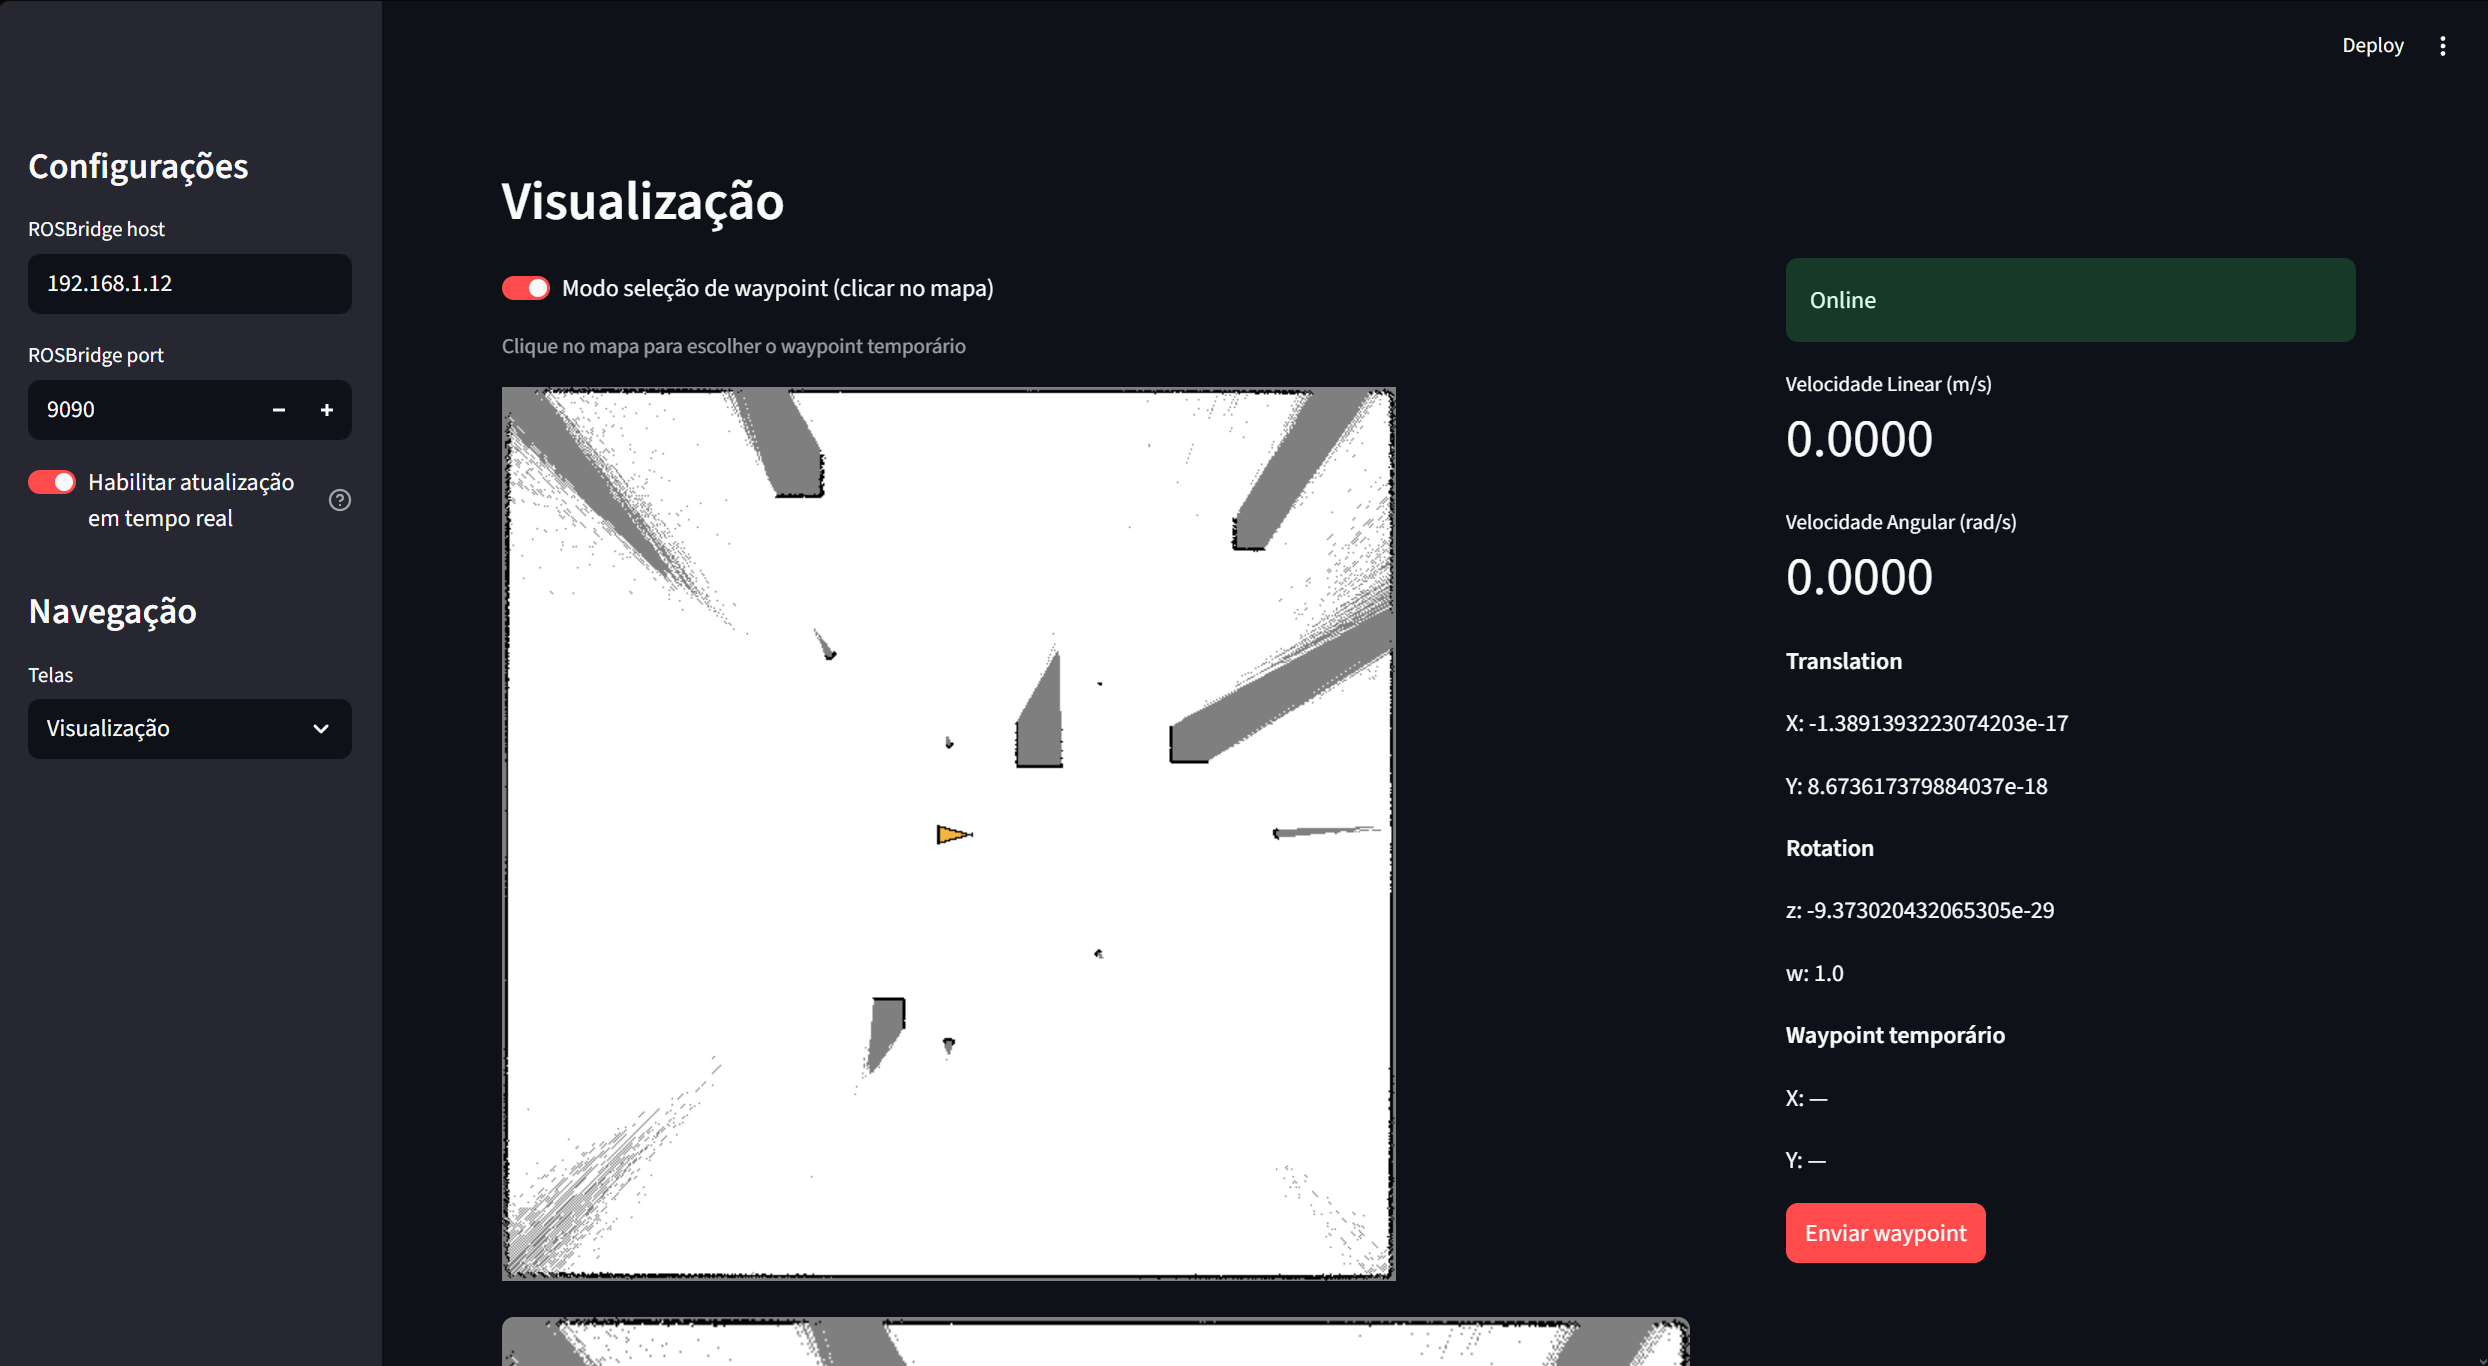
\includegraphics[width=\textwidth]{images/Visualizacao.png}
    \vskip0.5\baselineskip
    \captionof{figure}{Módulo de visualização da interface.}\label{fig:visualizacao}
\end{center}

% Para as figuras seguintes colocamos cada uma em página própria

\begin{center}
    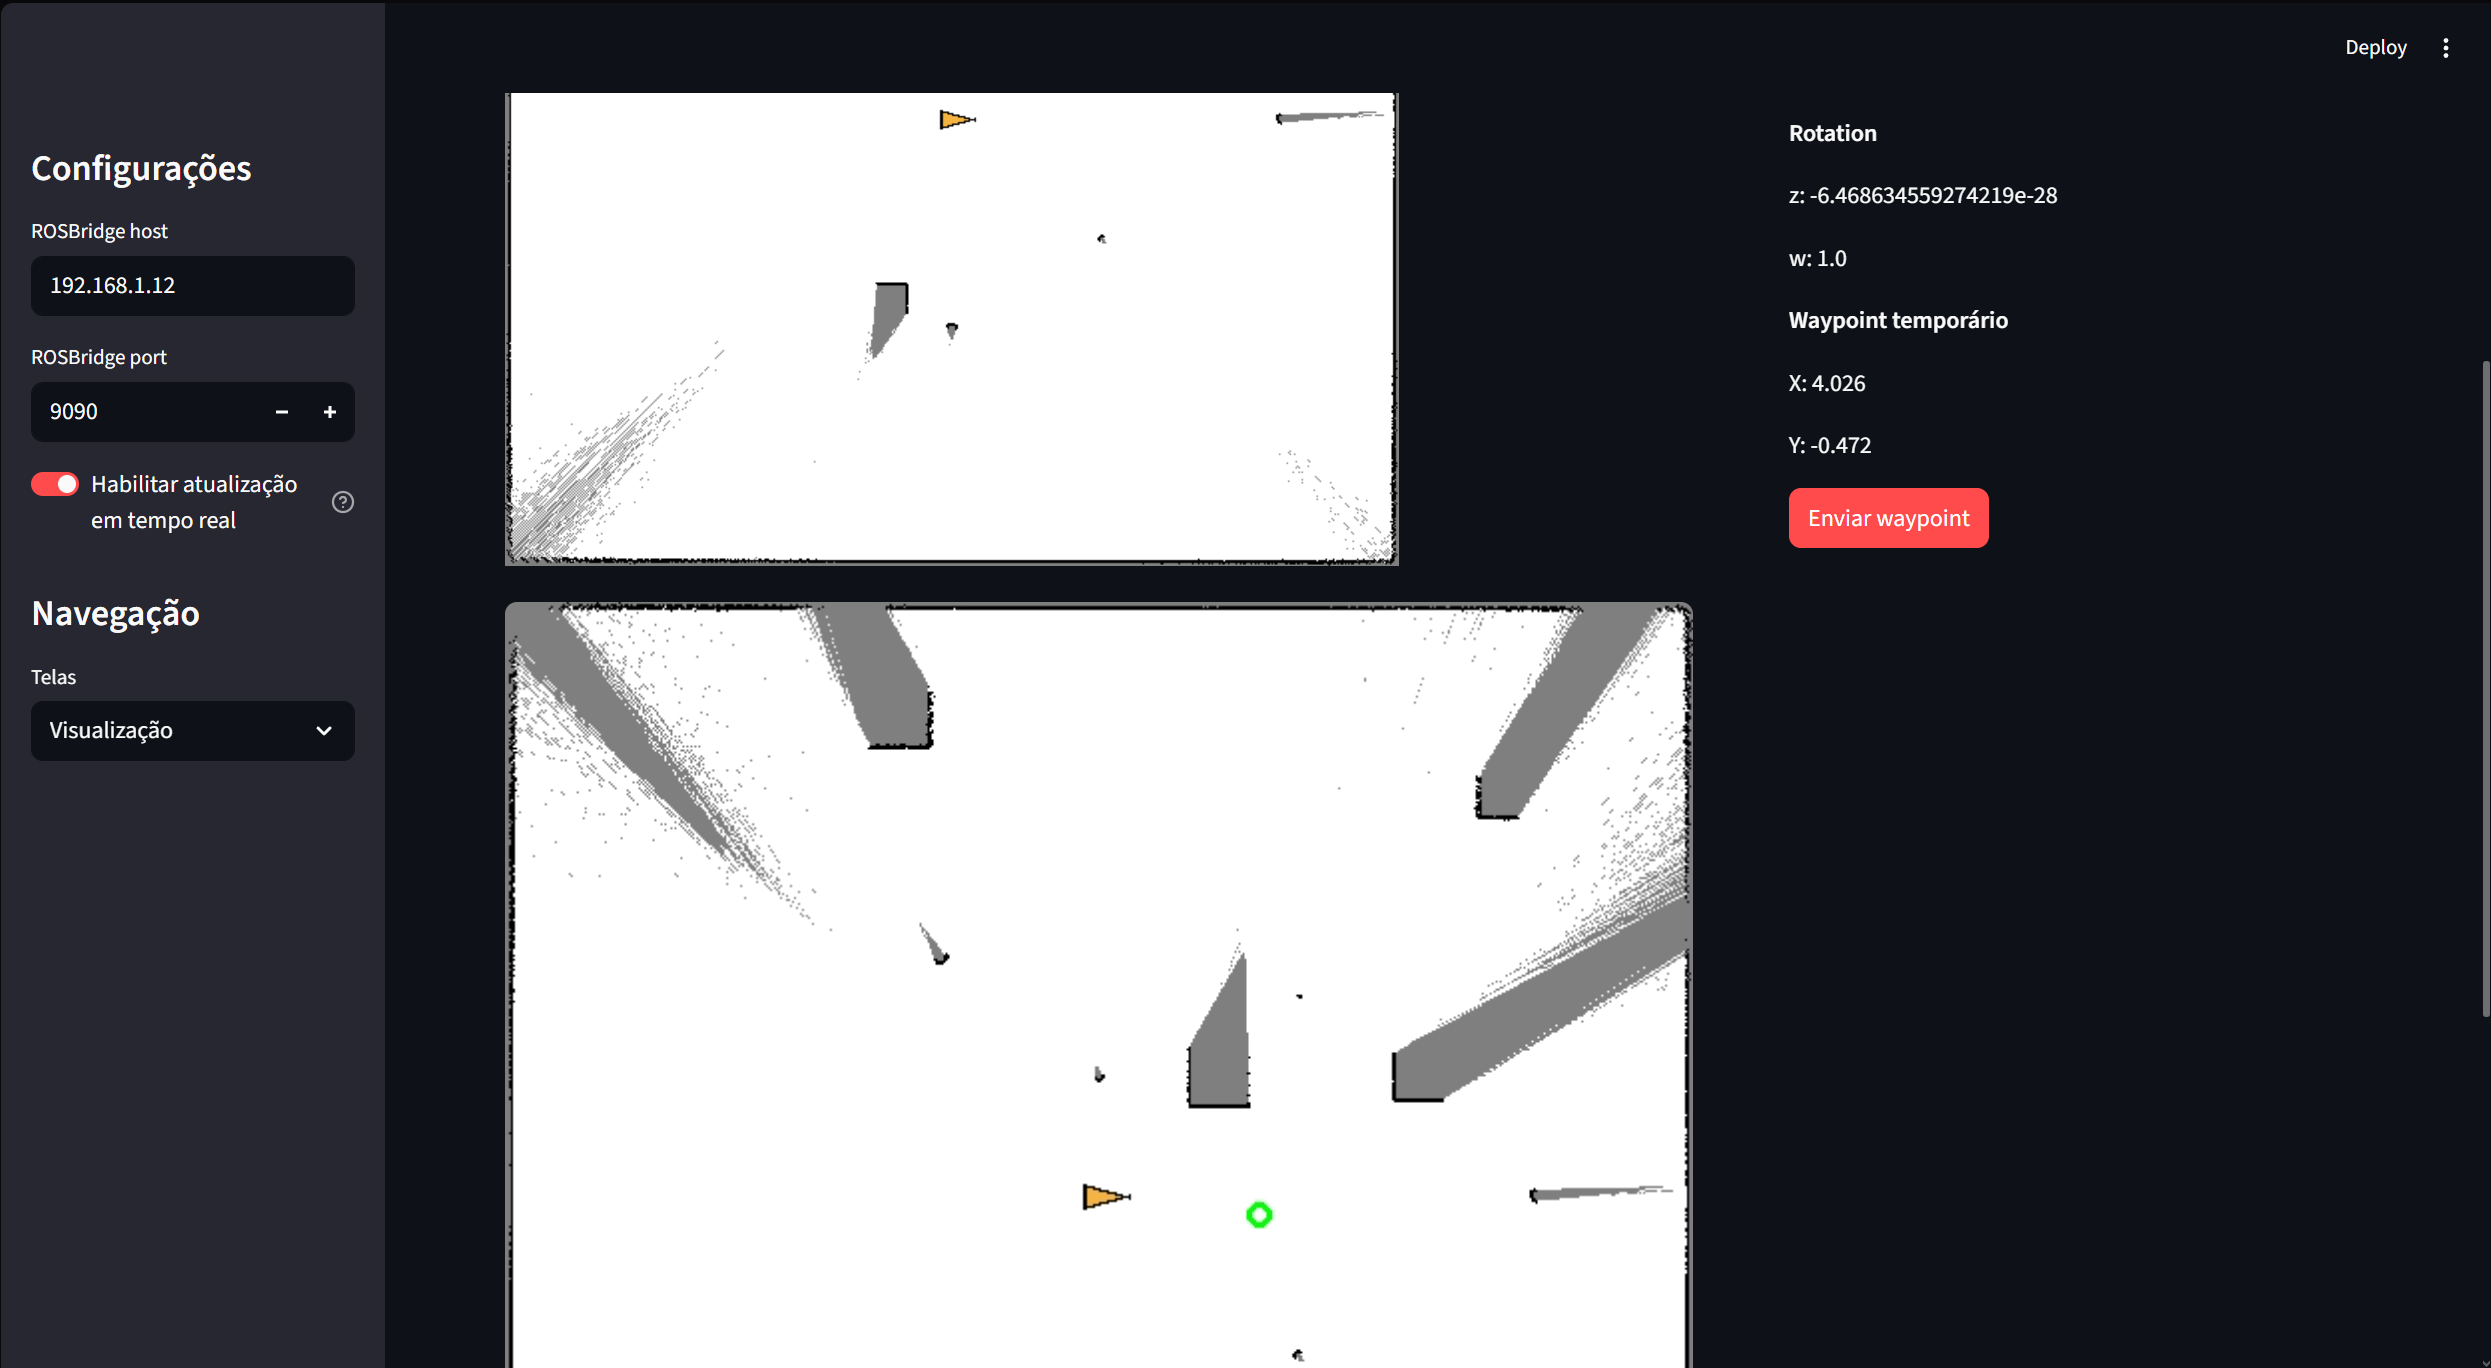
\includegraphics[width=\textwidth]{images/MostraWaypoint.png}
    \vskip0.5\baselineskip
    \captionof{figure}{Funcionalidade de definição de waypoint na interface.}\label{fig:mostra_waypoint}
\end{center}

\begin{center}
    \includegraphics[width=\textwidth]{images/RVizWaypoint.png}
    \vskip0.5\baselineskip
    \captionof{figure}{Envio de waypoint para o ROS e navegação automática do robô.}\label{fig:rvizwaypoint}
\end{center}

\begin{center}
    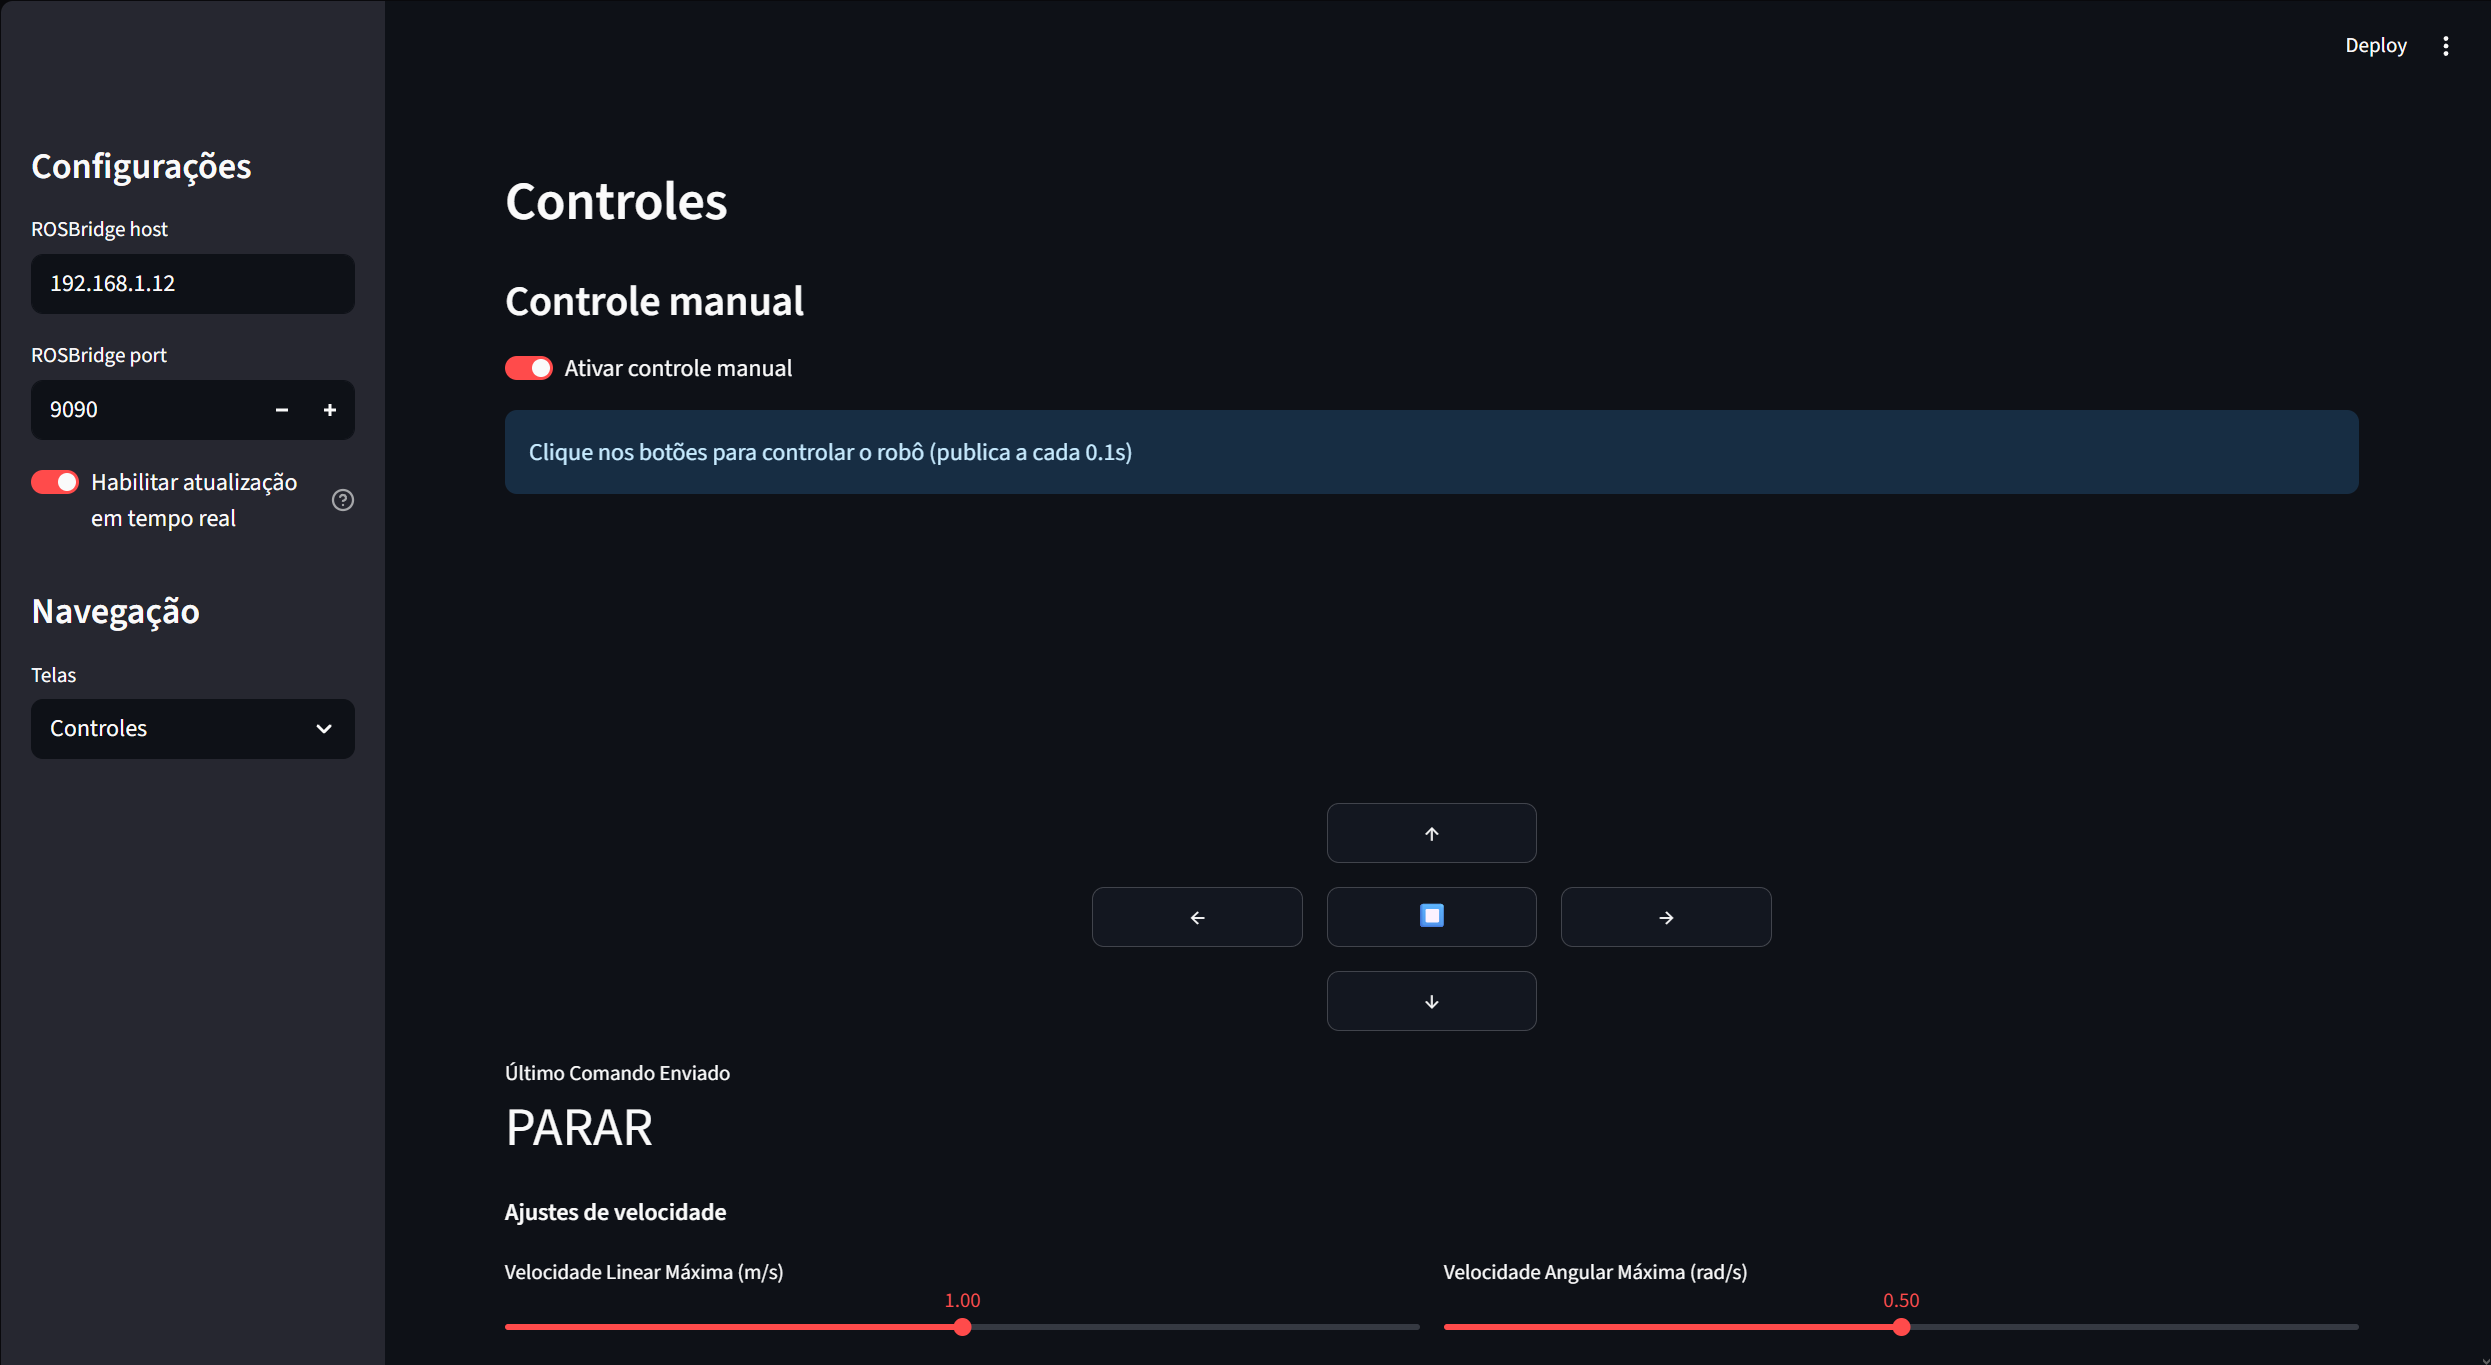
\includegraphics[width=\textwidth]{images/Controles.png}
    \vskip0.5\baselineskip
    \captionof{figure}{Módulo de controle da interface.}\label{fig:controle}
\end{center}

\begin{center}
    \includegraphics[width=\textwidth]{images/RVizControle.png}
    \vskip0.5\baselineskip
    \captionof{figure}{Envio de comandos de controle manual para o ROS.}\label{fig:rvizcontrole}
\end{center}


\end{document}
%Modelo para escrita de artigos científicos do Trabalho de Conclusão de Curso da Engenharia de computação
% Unoesc - Campus de Joaçaba

%Se você é novo no latex, um bom lugar para começar é
%https://pt.overleaf.com/learn

\documentclass[10pt,conference,twocolumn]{unoesc} 

% -------------------- Configuração para usar trecho de código --------------------

\usepackage[utf8]{inputenc}
\usepackage[T1]{fontenc}
\usepackage{listings}
\usepackage{xcolor}

\lstset{
    language=C++,
    basicstyle=\scriptsize\ttfamily, % Reduzido de \footnotesize para \scriptsize
    keywordstyle=\bfseries,
    stringstyle=\itshape,
    commentstyle=\slshape,
    numbers=left,
    numberstyle=\scriptsize, % Ajustado de \tiny para \scriptsize
    stepnumber=1,
    numbersep=8pt, % Aumentado de 5pt para 8pt
    showspaces=false,
    showstringspaces=false,
    frame=single,
    breaklines=true,
    breakatwhitespace=true,
    tabsize=2,
    xleftmargin=14pt, % Nova margem à esquerda para afastar o código da borda
    xrightmargin=5pt, % Nova margem à direita para balancear
    aboveskip=0.5em, % Reduz espaço acima do código
    belowskip=0.5em, % Reduz espaço abaixo do código
    literate={á}{{\'a}}1 {é}{{\'e}}1 {í}{{\'i}}1 {ó}{{\'o}}1 {ú}{{\'u}}1
             {ã}{{\~a}}1 {õ}{{\~o}}1 {â}{{\^a}}1 {ê}{{\^e}}1 {ô}{{\^o}}1
             {ç}{{\c{c}}}1 {à}{{\`a}}1,
}

% ---------------------------------------------------------------------------------

\usepackage{csquotes}
%Use esse arquivo para incluir novos pacotes

\usepackage[%usado para determinar medidas
top=1.78cm,
bottom=1.78cm,
left=1.65cm,
right=1.65cm,
headsep=0cm,
%showframe
]{geometry}
%\usepackage[justification=centering]{caption}
\usepackage{times}
\usepackage{enumitem}%redefinir espacos itemize
\usepackage{graphicx}
\usepackage{url,hyperref}
\usepackage[utf8]{inputenc}
\usepackage{float}%mais controle para manipular figuras
\usepackage{caption}%manipular legenda da figura e tabela
\usepackage{mathtools}%equacoes
\usepackage[hang,flushmargin]{footmisc} 
\usepackage{xcolor}
\usepackage{wrapfig} %usado para envolver figura com texto
%\usepackage[portuguese]{babel}
\usepackage{fancyhdr}%criacao do cabecalho
\usepackage{etoolbox}
\usepackage[export]{adjustbox}%mais controle para ajustar tamanho da tabela
\usepackage{comment}%ambiente para comentario
\usepackage{relsize} %usado por comandos \mathlarger
\usepackage{lipsum} 

%Referencia bibliografica
\usepackage[
    style=numeric,
    sorting=none,
    maxbibnames=10]{biblatex}
\addbibresource{referencia.bib}

%Idioma. Use "english" para trabalhos em inglês
\usepackage[brazil]{babel}
%Ajustes na legenda da figura. Incluindo espacamento apos a legenda
\captionsetup[figure]{labelformat={default},labelsep=period,font=footnotesize, name=\footnotesize{Fig.},justification=centering,singlelinecheck=false,belowskip=0\normalbaselineskip}
%\pagenumbering{gobble}

%Ajustes na legenda da tabela. 
\captionsetup[table]{labelformat={default},labelsep=newline,font={sc,footnotesize},justification=centering,singlelinecheck=false}

%\renewcommand{\headrulewidth}{0pt}

% Renomear a legenda de listings para Português sem usar caption (evita conflitos)
% Para o pacote `listings` (ambiente `lstlisting`)
\renewcommand{\lstlistingname}{Código}
% Renomear também o título da lista de listings, se usado
\renewcommand{\lstlistlistingname}{Lista de Códigos}

\makeatletter
\newcommand{\linebreakand}{%
  \baselineskip 
  \end{@IEEEauthorhalign}
  \hfill\mbox{}\par
  \mbox{}\hfill\begin{@IEEEauthorhalign}
}
\makeatother


%%%%%%%%%%%%%%%%%%%%%%%%%%%%%%%%%%%%%%%%%%%%%%%%%%%%%%%%%%%%%%%%%%%%%%%%%
%    Configuracaoes de Idioma
%    Considerando babel = brazil
%%%%%%%%%%%%%%%%%%%%%%%%%%%%%%%%%%%%%%%%%%%%%%%%%%%%%%%%%%%%%%%%%%%%%%%%% 

\addto\captionsbrazil{
  \renewcommand{\abstractname}{Abstract}
  \renewcommand{\tablename}{TABELA}
}

%considerando babel = english
\addto\captionsenglish{
  \renewcommand{\tablename}{TABLE}
}

\begin{document}


  \title{Interface Gráfica Integrada ao ROS para Telemetria e Parametrização de Robô Autônomo}
  \author
  {
    \IEEEauthorblockN{Rafael Corrêa Zart\\}
    \IEEEauthorblockN{Orientador: Kleyton Hoffmann\\}
    \IEEEauthorblockA{Universidade do Oeste de Santa Catarina - Unoesc\\
                    ACET - Área de Ciências Exatas e Tecnológicas \\
                    Curso de Engenharia de Computação - 
                    Campus de Joaçaba/SC}
  }

\maketitle

 \vspace{0.3cm}
  \begin{resumo}
     %%%%%%%%%%%%%% Não retirar este trecho
    \noindent\footnote{Trabalho de Conclusão de Curso apresentado ao Curso de Engenharia de Computação no segundo semestre de 2025, Área de Ciências Exatas e Tecnológicas da Universidade do Oeste de Santa Catarina como requisito parcial à obtenção do grau de bacharel em Engenharia de Computação.}
     %%%%%%%%%%%%%% Não retirar este trecho
     Este trabalho propõe o desenvolvimento de uma interface gráfica para telemetria e parametrização de robôs autônomos, integrada ao \textit{Robot Operating System} (ROS) por meio do protocolo ROSBridge. Utilizando a biblioteca Streamlit, a interface foi projetada para oferecer interação intuitiva, com visualização em tempo real de velocidade, posição e mapas 2D gerados por algoritmos SLAM (\textit{Simultaneous Localization and Mapping}), além de possibilitar ajustes de parâmetros operacionais e controle manual do robô. A metodologia empregada estrutura-se em três fases distintas: a caracterização do \textit{hardware}, o desenvolvimento modular e a validação em ambientes simulados (RViz) e reais. O desenvolvimento modular encontra-se concluído, com o módulo de visualização e de controle implementados. \textit{Scripts} de comunicação via ROSBridge estão operacionais e integrados à interface e funcionalidades como o mapeamento 2D com LiDAR (Light Detection and Ranging) e a implementação de \textit{waypoints} estão funcionando. Funcionalidades planejadas na primeira fase de desenvolvimento do trabalho de conclusão de curso, como plotar mapa 2D com nuvem de pontos e navegação autônoma por waypoints foram implementadas com sucesso, testes também foram realizados para validar a precisão de posicionamento no mapa e a eficácia da interface. O sistema demonstra potencial para aplicações em ambientes internos e semi-estruturados, contribuindo para a integração eficiente entre interfaces gráficas e sistemas robóticos.
     
  \end{resumo}
  
  \begin{palavraschave}
    aplicativo, app, interface gráfica, LiDAR, robô autônomo, ROSBridge, Streamlit, web.
  \end{palavraschave}
  
  \vspace{0.5cm}
  
  \begin{abstract}
  \noindent This work proposes the development of a graphical interface for telemetry and parameterization of autonomous robots, integrated with the \textit{Robot Operating System} (ROS) through the ROSBridge protocol. Using the Streamlit library, the interface was designed to offer intuitive interaction, with real-time visualization of velocity, position, and 2D maps generated by SLAM (\textit{Simultaneous Localization and Mapping}) algorithms, in addition to enabling adjustments of operational parameters and manual control of the robot. The methodology employed is structured in three distinct phases: \textit{hardware} characterization, modular development, and validation in simulated (RViz) and real environments. The modular development is concluded, with the visualization and control modules implemented. \textit{Scripts} for communication via ROSBridge are operational and integrated into the interface, and functionalities such as 2D mapping with LiDAR and the implementation of \textit{waypoints} are working. Planned features for the first development phase of the undergraduate thesis, such as plotting 2D maps with point clouds and autonomous navigation by waypoints were implemented successfully, tests were also conducted to validate the positioning accuracy on the map and the interface's effectiveness. The system demonstrates potential for applications in indoor and semi-structured environments, contributing to the efficient integration between graphical interfaces and robotic systems.
  \end{abstract}

  \begin{IEEEkeywords}
    application, app, Autonomous robot, graphical interface, LiDAR, ROSBridge, Streamlit, web.
  \end{IEEEkeywords}
  
    \vspace{0.5cm}
\section{Introdução}

% A introdução deve conter uma visão geral sobre o tema, uma explicação geral do que o trabalho pretende com ou sem suporte de trabalhos correlatos. Nesta seção também deve estar clara a descrição do problema, a justificativa, os objetivos e a organização do trabalho.

% ----------------------------------- Contextualização do Tema -----------------------------------

A robótica autônoma tem se tornado cada vez mais presente em aplicações críticas que abrangem desde operações em ambientes extremos até tarefas cotidianas de automação. Estudos recentes na área destacam que a eficácia operacional desses sistemas depende fundamentalmente da integração harmoniosa entre interfaces de usuário bem projetadas e arquiteturas de controle confiáveis. Essa combinação estratégica não apenas possibilita uma interação mais intuitiva entre humanos e máquinas, mas também garante a execução autônoma eficiente de missões complexas, mantendo sempre a capacidade de supervisão e intervenção humana quando necessária \cite{IntroAR}.
 
% --------------------------------

Eu gosto de estudar robótica autônoma, e tenho interesse em desenvolver uma interface gráfica para controle de robôs autônomos, integrando-a com o ROS (Robot Operating System) para facilitar a comunicação e o controle em tempo real. O objetivo é criar uma plataforma que permita a visualização de dados sensoriais, a definição de metas de navegação e o controle manual do robô, utilizando tecnologias modernas de desenvolvimento de interfaces. A motivação para este projeto surge da necessidade de melhorar a interação entre humanos e robôs, tornando o controle mais acessível e eficiente, especialmente em ambientes internos onde a navegação autônoma pode ser desafiadora \cite{IntroROS}.

% -------------------------------- Estado da Arte / Revisão Breve --------------------------------

Estudos na área de robótica autônoma demonstram que os sistemas de controle para essas plataformas normalmente empregam técnicas consolidadas como controladores PID (proporcional integral derivativo), lógica \textit{fuzzy} e redes neurais \cite{KleytinhoBasico}. No âmbito das interfaces gráficas, observa-se uma diversidade de abordagens, desde soluções \textit{desktop} baseadas em ROS até interfaces \textit{mobile} para Android, cada uma com seus requisitos específicos de integração \cite{robo2wd, Teleoperacao}. Um desafio comum identificado na literatura é a dificuldade em estabelecer uma comunicação eficiente entre o núcleo de controle do robô e diferentes tipos de interfaces gráficas, frequentemente resultando em atrasos indesejados ou perda de sincronismo nos dados, independentemente da plataforma utilizada \cite{IntroROS}.

% ------------------------------------- Problema de Pesquisa -------------------------------------

A integração entre interfaces gráficas e sistemas de controle representa um dos principais desafios na robótica autônoma, impactando diretamente a eficácia operacional das plataformas robóticas \cite{IntroAR, IntroROS}. Este trabalho propõe uma solução que combina interfaces intuitivas com algoritmos de controle adaptativos, atendendo aos requisitos críticos de usabilidade e desempenho em sistemas robóticos autônomos.

% ---------------------------------------- Justificativa -----------------------------------------

A relevância desta pesquisa se manifesta em três aspectos principais: a otimização da interação humano-robô, essencial para sistemas de controle e supervisão; a contribuição para arquiteturas padronizadas, facilitando a replicabilidade de soluções; e a aplicação em cenários complexos, como navegação em ambientes dinâmicos e inspeção automatizada \cite{IntroROS}.

% ------------------------------------------ Trekking --------------------------------------------

A modalidade \textit{Trekking} em competições robóticas desafia os robôs a navegarem autonomamente em terrenos irregulares, superando obstáculos utilizando fusão de dados sensoriais (LIDAR, IMU e câmeras) para mapeamento 3D e tomada de decisão \cite{KleytinhoBasico}. As regras avaliam não apenas a conclusão do percurso, mas também critérios como suavidade de movimento, eficiência energética e precisão de posicionamento (tolerâncias $\leq$ 5~cm). Essas regras tornam o ambiente de competição um \textit{benchmark} ideal para validar sistemas robóticos integrados, já que exige interfaces gráficas responsivas, algoritmos de controle adaptativos e comunicação robusta, requisitos que demonstram transferibilidade direta para aplicações práticas como agricultura de precisão e inspeção de infraestruturas \cite{KleytinhoBasico}.

% ------------------------------------------ Objetivos -------------------------------------------

O objetivo central do meu trabalho consiste no desenvolvimento de uma plataforma robótica integrada, com dois focos específicos: implementação de uma interface gráfica otimizada para controle robótico e validação em ambientes característicos de aplicações robóticas \cite{IntroAR, IntroROS}.

% ------------------------------------- Metodologia (Breve) --------------------------------------

Partindo da plataforma robótica já adquirida para o projeto, o desenvolvimento seguirá uma abordagem prática em três etapas integradas. Na fase inicial, será realizada a caracterização detalhada do \textit{hardware} disponível, mapeando suas capacidades e limitações para orientar o projeto da interface gráfica e dos algoritmos de controle. A implementação adotará uma arquitetura modular, com desenvolvimento paralelo e teste individual de cada subsistema (interface móvel, núcleo de controle e módulo de comunicação) seguindo padrões de interoperabilidade consagrados na área. A etapa final consistirá na integração progressiva e validação do sistema completo, com testes em condições reais de operação que aproveitem plenamente as capacidades da plataforma física disponível, assegurando robustez e desempenho adequados às aplicações planejadas.

% ------------------------------------- Estrutura do Artigo --------------------------------------

Este artigo está estruturado em sete seções. Na seção I, foi introduzido o tema da robótica autônoma e os desafios na integração interface-controle, com os objetivos do trabalho. Na seção II, foram abordados os conceitos teóricos fundamentais sobre navegação autônoma, algoritmos de controle e protocolos de comunicação. Na seção III, foram examinadas pesquisas anteriores sobre sistemas similares, identificando lacunas a serem superadas e ideias a serem exploradas. Na seção IV, foi descrita a metodologia em três fases: caracterização do hardware, desenvolvimento modular e validação. Na seção V, foram mostrados os resultados dos testes de desempenho do sistema. Na seção VI, foram apresentados os resultados finais em condições reais de operação. Na seção VII, foram destacadas as conclusões e sugestões para trabalhos futuros.
\section{Referencial Teórico}
\label{sec:referencial}

Neste capítulo são apresentadas as tecnologias: robótica autônoma, telemetria, mapeamento, planejamento de trajetória e API, que foram utilizadas para o desenvolvimento do trabalho, com o objetivo de familiarizar o leitor a ter uma leitura mais compreensiva do mesmo.


\subsection{Robótica Autônoma}
A robótica autônoma tem evoluído continuamente, tornando-se cada vez mais relevante no cenário tecnológico atual. A capacidade dos robôs autônomos substituírem humanos em atividades perigosas ou repetitivas justifica os investimentos na área. Competições e projetos educacionais desempenham papel fundamental na formação de profissionais e no estímulo ao interesse pela robótica \cite{RoboAutonomo}.

Alguns dos principais desafios são navegação, planejamento de trajetória, localização e desvio de obstáculos \cite{AMRChallenges}. Os sistemas de navegação de robôs móveis dependem do nível de abstração da representação do ambiente \cite{Mapeamento}. Para determinar com precisão a posição e a orientação do robô móvel, é essencial que o ambiente seja modelado em uma estrutura simples e compreensível.
A parte desafiadora da localização é estimar a posição do robô e a orientação da qual essa informação pode ser obtida de sensores e outros sistemas. Para lidar com o desafio da localização, uma boa técnica deve ser desenvolvida para tratar erros, fatores de interferência, medições incorretas e estimativas imprecisas \cite{Odometria}. Desvio de obstáculos é uma tarefa essencial no campo da robótica, pois é fundamental que o robô alcance seu destino sem ser bloqueado por qualquer obstáculo ou sofrer colisões em seu trajeto \cite{PlanejamentoTrajetoria}. Por esse motivo, algoritmos livres de colisão são um requisito indispensável para robôs móveis autônomos \cite{IntroAR, AMRChallenges}.

Os robôs autônomos têm aplicações variadas: podem atuar desde o campo, monitorando lavouras, até ambientes industriais, seja atuando em processos produtivos como linhas de montagem e gestão logística de estoques em armazéns.

\subsection{ROS}
O Robot Operating System (ROS) é um conjunto de bibliotecas de \textit{software} e ferramentas que auxiliam no desenvolvimento de aplicações robóticas. De \textit{drivers} a algoritmos de ponta, e com poderosas ferramentas para desenvolvedores, o ROS oferece o que você precisa para o seu próximo projeto de robótica. E tudo isso é de código aberto \cite{ROS_Website}.

O ROS vai além de ser apenas um conjunto de bibliotecas, ele funciona como um ecossistema robusto que padroniza a comunicação entre diferentes componentes de software em um robô. Ele oferece um modelo de programação distribuída, onde múltiplos nós (programas executáveis independentes) podem se comunicar enviando e recebendo mensagens através de tópicos. Isso permite que desenvolvedores de diversas áreas colaborem em um mesmo projeto robótico, com cada um focando em um módulo específico (como navegação, percepção ou controle), e o ROS garantindo a integração.

\subsection{Telemetria}
A palavra telemetria é a união de duas palavras gregas. \textit{Tele} significa longe e 
\textit{meter} significa medir. Por isso, telemetria significa realizar medições à distância, ou em local remoto. Os ingredientes essenciais de qualquer sistema de telemetria incluem pelo menos um sensor, uma antena transmissora de baixo ganho, uma antena receptora de alto ganho, um receptor e um mostrador \cite{Telemetria}. 

Teste de veículos foi uma das primeiras aplicações da telemetria. Inicialmente, não tripulados, como mísseis guiados, requeriam telemetria, para que os engenheiros soubessem o que se passava dentro do míssil. Veículos tripulados também requeriam telemetria para medir parâmetros, tais como fadiga da asa, que não eram perceptíveis aos tripulantes 
\cite{Telemetria}.

\subsection{Mapeamento e Planejamento de Trajetória}
A técnica geral de \textit{roadmap} para planejamento de trajetórias consiste em capturar a conectividade do espaço livre do ambiente em uma rede de curvas de uma dimensão, denominada \textit{roadmap}. Uma vez que esta rede tenha sido obtida, ela é vista como um conjunto padrão de caminhos. O planejamento de trajetórias reduz-se então a conectar as posições iniciais e finais do robô ao \textit{roadmap} e buscar neste um caminho entre esses dois pontos, conforme pode ser observado na Figura \ref{fig:roadmap} \cite{PlanejamentoTrajetoria}.

\begin{figure}[h]
    \centering
    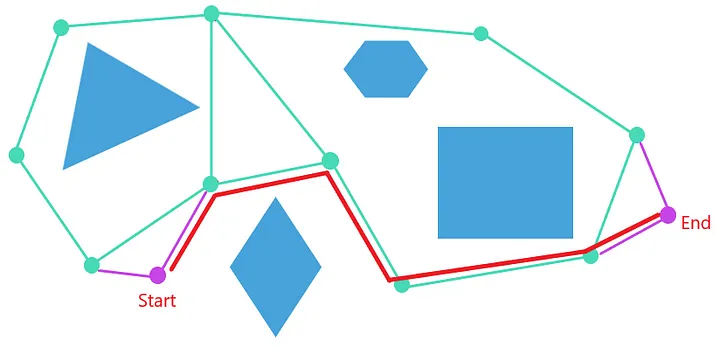
\includegraphics[width=0.45\textwidth]{images/RoadmapRT.png}
    \caption{Gráfico de navegação \textit{roadmap} para encontrar a melhor rota.}
    \label{fig:roadmap}
    % Referência: https://arushi-khokhar.medium.com/probabilistic-roadmap-prm-for-path-planning-in-robotics-d4f4b69475ea
\end{figure}

Quando não há um mapa do ambiente obtido a \textit{priori}, é preciso construir o mapa durante a navegação. Nesse caso, técnicas de localização e mapeamento simultâneo (SLAM) são usadas \cite{SLAM}.

Resolver o problema de SLAM envolve a estimação da trajetória do robô e do mapa do ambiente enquanto o robô se desloca. Ao longo da movimentação do robô em poses sequenciais desconhecidas \( x_{1:t} = x_1, x_2, \ldots, x_t \) em um mapa desconhecido \( m \), são obtidas uma sequência de odometria \( u_{1:t} = u_1, u_2, \ldots, u_t \) e observações do ambiente \( z_{1:t} = z_1, z_2, \ldots, z_t \). O problema SLAM requer a obtenção da distribuição de probabilidades dada pela Equação 1, considerando que \( x_0 \) é a posição inicial do robô \cite{Mapeamento}.

O Cartographer é um sistema de SLAM eficiente que opera em dois níveis: localmente ajusta a pose do robô em submapas usando um \textit{scan matcher} (Ceres), enquanto globalmente refina a localização combinando todos os submapas em um mapa maior \cite{Cartographer, Ceres}. Sua principal vantagem é a flexibilidade, com suporte a múltiplos sensores e resoluções, e a eficiência computacional que permite operação em tempo real \cite{NVIDIA_JetsonOrinNano}.

Existe uma dificuldade intrínseca em conciliar as medições de localização com a posição verdadeira do dispositivo após longos períodos de navegação. O desafio origina-se na imprecisão dos sensores de medidas de odometria (ex: sonares, lasers e câmeras) devido às limitações físicas e imprevisibilidades do sistema \cite{Odometria}.

\subsection{API}
APIs (Interface de Programação de Aplicações) simplificam e aceleram o desenvolvimento de aplicativos e \textit{software}, permitindo que os desenvolvedores integrem dados, serviços e recursos de outros aplicativos, em vez de desenvolvê-los do zero. As APIs também oferecem aos proprietários de aplicativos uma maneira simples e segura de disponibilizar os dados e as funções dos aplicativos para os departamentos da organização. Os proprietários de aplicativos também podem compartilhar ou comercializar dados e funções para parceiros de negócios ou terceiros \cite{IbmAPI}.

As APIs permitem o compartilhamento apenas das informações necessárias, mantendo ocultos outros detalhes internos do sistema, o que auxilia na segurança do sistema. Os servidores ou dispositivos não precisam expor totalmente os dados: as APIs permitem o compartilhamento de pequenos pacotes de dados, relevantes para a solicitação específica \cite{IbmAPI}.

Podem existir vulnerabilidades de segurança devido à implementação da API. Por exemplo, a falha em verificar o tamanho dos \textit{inputs} na sua API pode permitir que um atacante derrube seu servidor ao enviar um \textit{input} extremamente grande que consuma toda a memória disponível - um tipo de ataque de negação de serviço (DoS) \cite{APISecurity}.

ROSBridge é uma especificação de protocolo de rede em camada de aplicação para o ROS (\textit{Robot Operating System}) que enfatiza o modelo cliente/servidor. Especificamente, o ROSBridge permite que clientes publiquem e escrevam mensagens em tópicos e invoquem serviços no ambiente de execução do servidor. O protocolo transporta mensagens formatadas em JSON por meio de \textit{sockets} TCP ou \textit{WebSockets} \cite{ROSBridge}.

No trecho de código \ref{lst:conexao_websocket} a classe roslibpy.ros é instanciada com o IP do dispositivo ROS e também a porta padrão para comunicação WebSocket, e o método client.run() inicia a conexão com o servidor ROS.   

\begin{lstlisting}[caption={Configuração da Conexão WebSocket com ROSBridge},label={lst:conexao_websocket}]
    import roslibpy
    
    # Configura a conexão WebSocket com o ROSBridge
    rosbridge_ws_url = '192.168.137.150'  # IP do dispositivo ROS
    client = roslibpy.Ros(host=rosbridge_ws_url, port=9090)

    # Conecta ao ROS
    client.run()
\end{lstlisting}
    
\subsection{Articulação das Tecnologias}
As tecnologias apresentadas neste referencial teórico articulam-se de forma coerente e complementar na solução desenvolvida. A robótica autônoma fornece a base conceitual para o sistema, enquanto as técnicas de telemetria e os protocolos de comunicação (ROSBridge) garantem a troca eficiente de dados entre os componentes. O SLAM e os algoritmos de planejamento de trajetória permitem a navegação autônoma, sendo acessíveis ao usuário através da interface desenvolvida com \textit{frameworks} modernos. As APIs, por sua vez, atuam como elemento integrador, possibilitando a comunicação segura entre a aplicação e o sistema robótico. Esta sinergia tecnológica resulta em uma plataforma completa que aborda desde a percepção ambiental até a interação com o usuário final, cumprindo os objetivos propostos de forma integrada e eficiente.
\section{Trabalhos Correlatos}
\label{sec:trabalhos}

% Sobre o que é, tecnologia utilizada, para que foi usado.
% O que faz?
% Por que é parecido?

Lima e Silva (2022) \cite{robo2wd} propuseram um sistema que viabiliza a programação e controle de um robô carro 2WD (duas rodas), utilizando Unity e C\# para desenvolver o aplicativo. O aplicativo tem as funções de ser servidor para múltiplos dispositivos e fornecer controle manual sobre um robô. Essa proposta se assemelha ao projeto do meu trabalho ao utilizar um aplicativo para o controle do robô autônomo.

Zago (2018) \cite{TelemetriaCompeticao} desenvolveu um sistema de telemetria sem fio para robôs de combate utilizando a tecnologia \textit{Bluetooth} para comunicação e o sistema operacional Android com um aplicativo para monitoramento do robô. O sistema de telemetria foi desenvolvido de uma maneira que não afeta diretamente  a funcionalidade, ou seja, o robô continua funcionando se o sistema de medição sofrer algum dano. Esse estudo se alinha a este trabalho pois utiliza a telemetria para comunicação com o robô e também utiliza um aplicativo para controle dos dados.

Werneck et al. \cite{TelemetriaSolar} elaboraram um sistema de telemetria para uma embarcação movida a energia solar para monitorar dados elétricos e de desempenho do barco solar em tempo real. Utilizaram um ESP32 para processamento, LoRa para transmissão de dados a longas distâncias, .NET para desenvolvimento da interface e outras tecnologias. O sistema mede e transmite dados para uma estação terrestre via LoRa ou conexão 4G. Os dados são processados e exibidos em uma interface gráfica desenvolvida em .NET para monitoramento e análise. Este projeto é semelhante ao meu estudo por utilizar tecnologias de telemetria e interface gráfica para monitoramento em tempo real de parâmetros do sistema embarcado.

Pico et al. \cite{Teleoperacao} propuseram um sistema de alarme e teleoperação em tempo real para falhas de navegação autônoma, comparando ROS 1 e ROS 2. O sistema integra uma interface web baseada em Vue.js e um \textit{joystick} com \textit{feedback} háptico para monitorar e controlar robôs em ambientes dinâmicos. A arquitetura utiliza sensores LiDAR (\textit{Light Detection and Ranging}), câmeras RGB-D e IMU para detectar colisões iminentes ou instabilidades em terrenos irregulares, acionando alertas visuais e vibrações no \textit{joystick}. Essa proposta se assemelha ao meu trabalho ao empregar uma interface gráfica para teleoperação e integração multimodal de sensores, com destaque para a comunicação via ROSBridge.

Perin et al. \cite{KleytinhoBasico} desenvolveram um robô móvel autônomo para competições ao ar livre, utilizando um chassi comercial adaptado. O sistema de percepção do robô é composto por um sensor de orientação de 9 eixos e um encoder incremental para localização e odometria. Para o controle de trajetória e velocidade, foram implementados controladores PID em C++, e o sistema foi simulado em um ambiente ROS integrado com a plataforma V-REP antes da implementação física. A proposta se assemelha ao meu trabalho ao empregar um sistema embarcado para o controle autônomo de um robô, com a particularidade de focar na navegação por coordenadas pré-definidas em campo aberto.
\section{Metodologia}
\label{sec:metodologia}

% ------------------------------- Apresentação Geral da Metodologia ------------------------------

Este trabalho adota uma abordagem metodológica estruturada em três fases para desenvolver uma interface gráfica intuitiva, estabelecer uma conexão robusta e validar o sistema em ambientes operacionais reais, com foco em robôs autônomos em ambientes internos e semi-estruturados. 

% --------------------------- Estratégia de Desenvolvimento e Validação --------------------------

A metodologia inicia com a análise do \textit{hardware} comercial disponível e a definição de requisitos técnicos. Em seguida, avança-se para o desenvolvimento paralelo dos subsistemas. Isso inclui a interface gráfica de usuário (GUI) com testes de usabilidade, a conexão robô-interface e os protocolos de comunicação via ROSBridge, conforme ilustrado na Figura \ref{fig:diagram}. O foco desta etapa é priorizar a exibição em tempo real de parâmetros essenciais, como posição, orientação e estado do sistema. Dessa forma, não são incorporados recursos avançados de aprendizado de máquina ou análise preditiva. A etapa final consiste em testes de integração e validação em ambientes simulados (RViz) e reais, limitados pelo período de desenvolvimento do trabalho acadêmico, o que restringe a quantidade de cenários avaliados.
% ---------------------- Abordagem Sequencial: Eficiência e Escalabilidade -----------------------

Essa abordagem sequencial assegura a verificação individual de cada componente antes da integração final, o que garante a eficiência operacional nas condições práticas previstas. Além disso, tal estrutura abre oportunidades para futuras expansões, como o desenvolvimento de componentes personalizados ou aplicações em ambientes externos.

\subsection{Análise do Hardware}
% -------------------------------- Caracterização do Hardware --------------------------------

A primeira fase da metodologia caracteriza o NVIDIA Jetson Orin Nano Developer Kit, plataforma do sistema robótico. O kit inclui um módulo Jetson Orin Nano 8GB com GPU NVIDIA Ampère (1024 núcleos CUDA), CPU de 6 núcleos e 8GB de memória LPDDR5, oferecendo até 40 TOPS (\textit{Tera Operations Per Second}) para aplicações de robótica. Sensores como LiDAR, IMU de 6 eixos e ultrassônicos, conectados via USB 3.2 Tipo-A ou conector de 40 pinos, suportam mapeamento 2D e navegação. Dois conectores MIPI CSI permitem câmeras para visão computacional. O armazenamento usa microSD ou SSD NVMe (M.2 Key-M). A comunicação ocorre via Wi-Fi, integrando com o ROS via ROSBridge \cite{NVIDIA_JetsonOrinNano}.


%Requisitos técnicos

%verificar 3D lidar ok

\subsection{Arquitetura do Sistema}

\begin{figure*}[htpb]
    \centering
    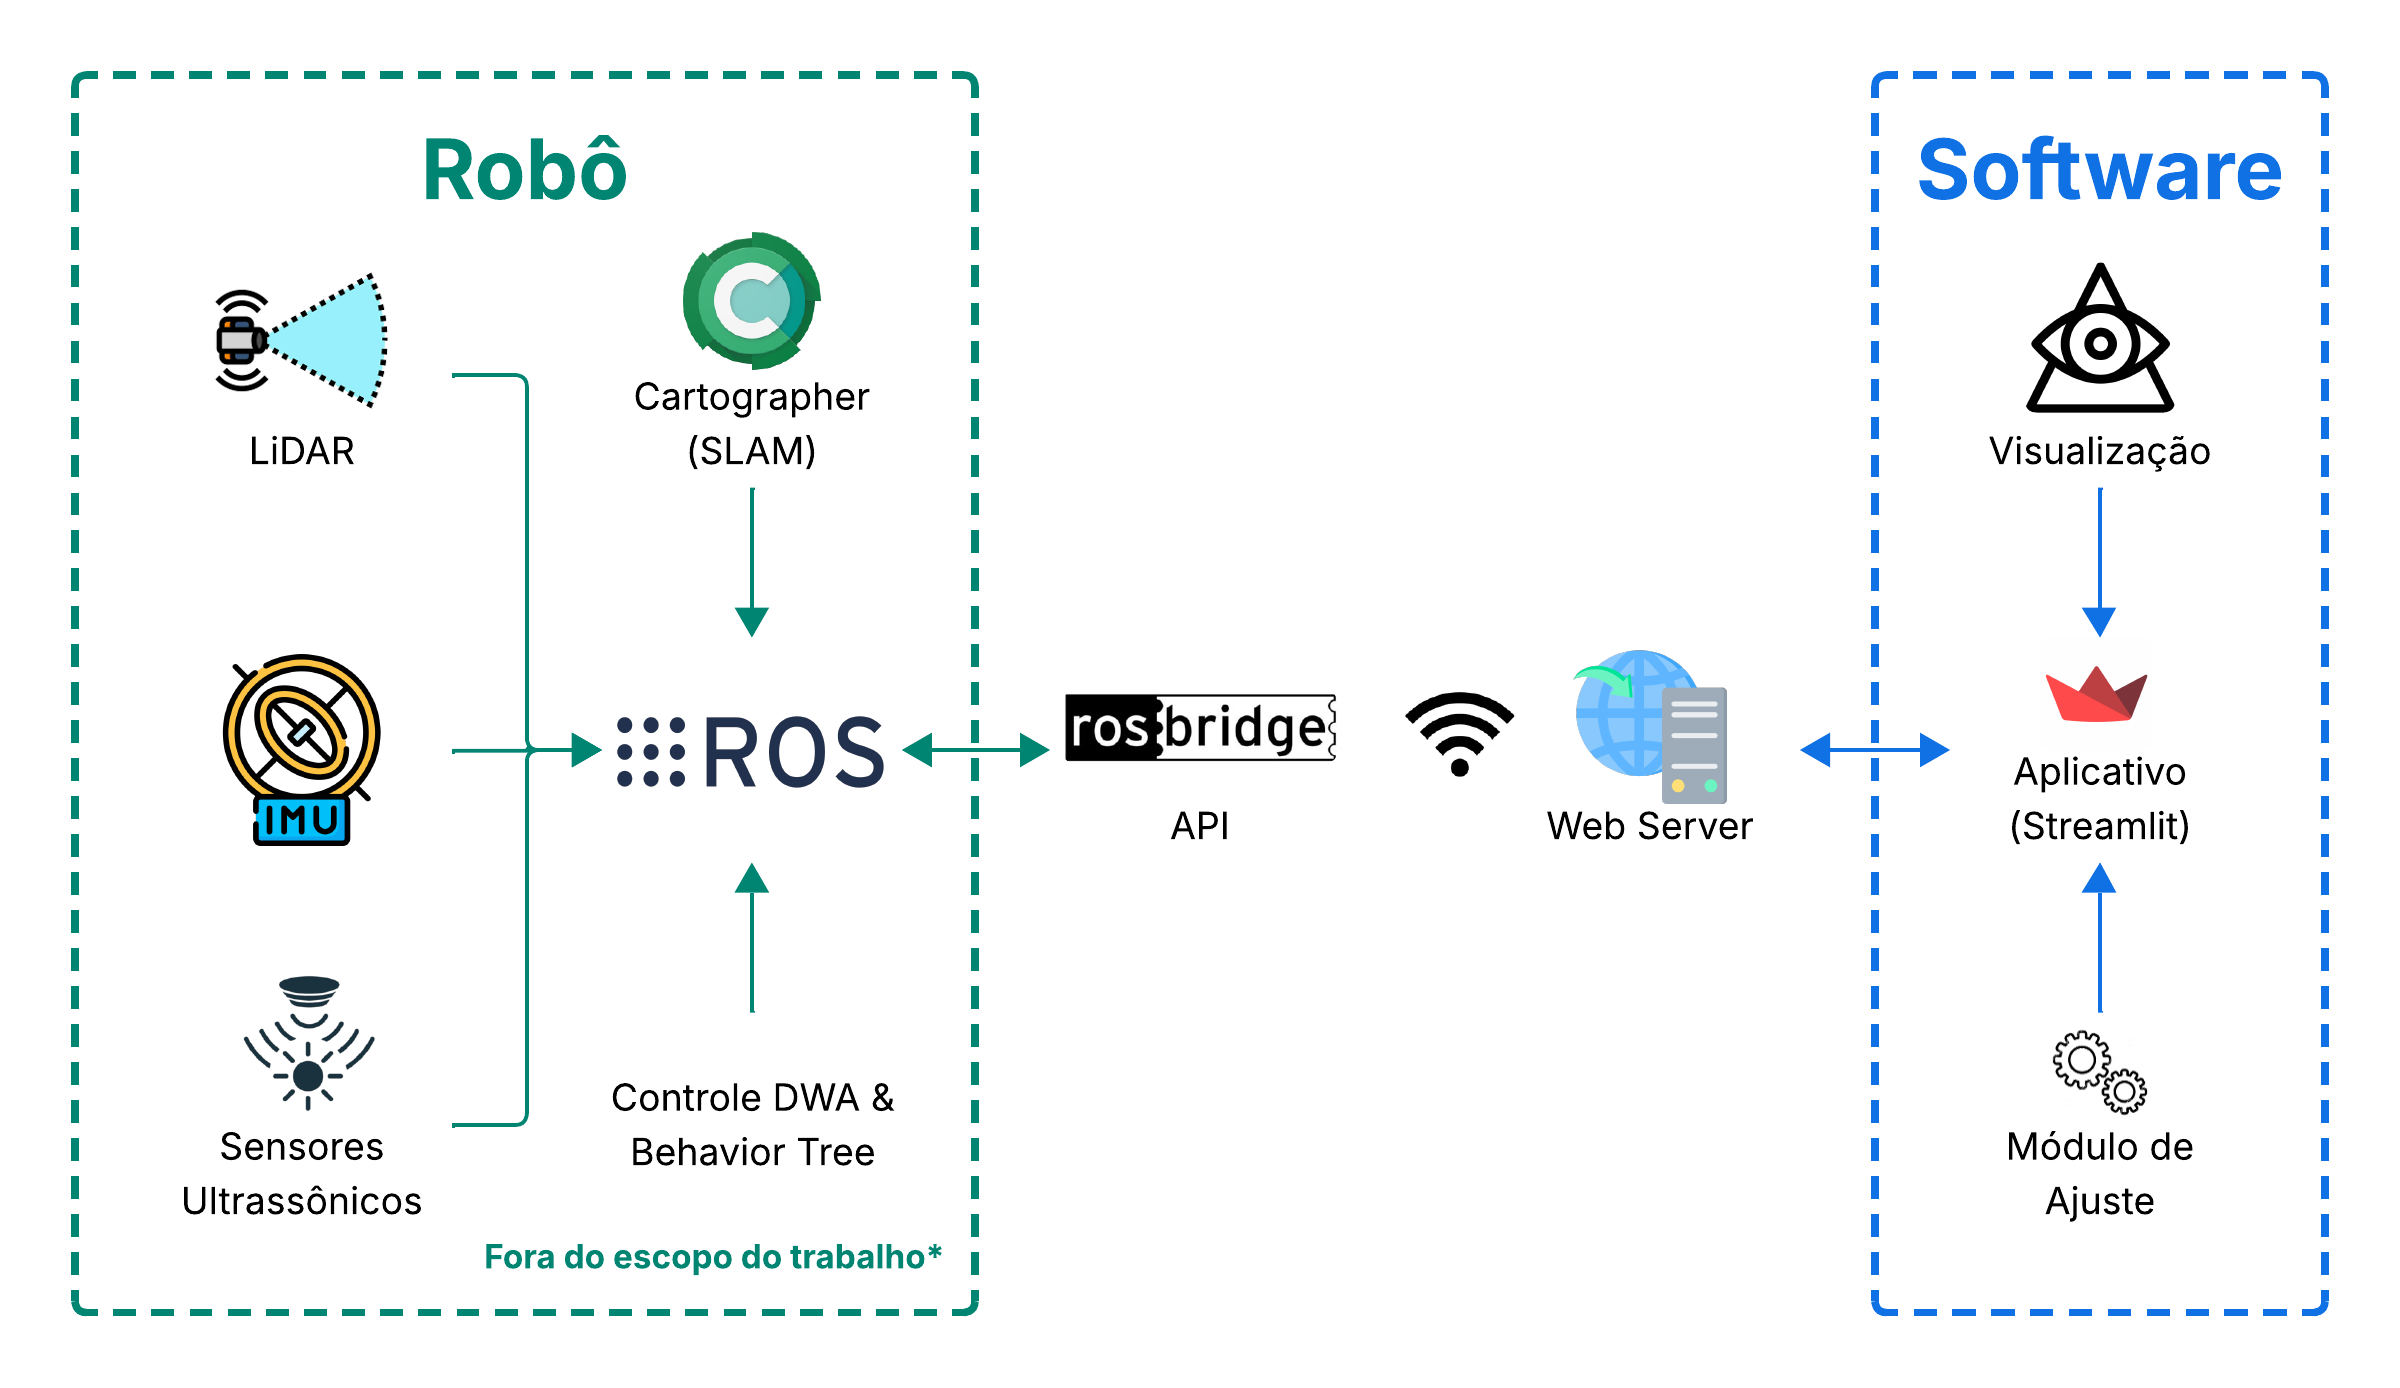
\includegraphics[width=\textwidth]{images/Diagrama_Arq.png}
    \caption{Diagrama da arquitetura do sistema.}
    \label{fig:diagram}
\end{figure*}

%fazer a chamada da figura no primeiro parágrafo. ok

O sistema robótico é projetado com uma arquitetura modular distribuída em três camadas principais, concebida para oferecer alta escalabilidade e flexibilidade na integração com diferentes plataformas robóticas e configurações de sensores. Na camada de percepção, os sensores atuam como os órgãos sensoriais do robô: um LiDAR para mapeamento 3D do ambiente, uma IMU de 6 eixos para medição inercial e sensores ultrassônicos para detecção de obstáculos próximos. 

A camada de processamento reside em um computador embarcado que opera o ROS (\textit{Robot Operating System}). Importante ressaltar que, apesar da nomenclatura, o ROS funciona como um \textit{framework} de software para robótica, e não como um sistema operacional em si. Essa camada estabelece a comunicação com os demais componentes através do ROSBridge, gerenciando a telemetria (incluindo dados de velocidade e status do sistema) e a integração direta com a interface. A ampla utilização do ROS como padrão na indústria e academia contribui para a facilidade de integração com uma diversidade de plataformas robóticas e dispositivos, o que intrinsecamente melhora a escalabilidade da arquitetura.

Na camada de interface com o usuário, o Streamlit \cite{Streamlit} fornece uma aplicação web acessível via navegador, exibindo dados de telemetria em tempo real e permitindo o controle manual quando necessário. A interface se conecta ao ROS através do ROSBridge, garantindo baixa latência na troca de comandos. Medidas de segurança como autenticação de usuário e criptografia serão implementadas para proteger a comunicação \cite{Streamlit}.

O fluxo de dados segue um ciclo contínuo: os sensores enviam informações para o ROS, que processa e toma decisões de navegação, enquanto a interface exibe os dados, recebe e envia comandos ao usuário. Os módulos são projetados para operar de forma independente em caso de falha pontual. A arquitetura desacoplada e a comunicação padronizada via ROS conferem ao sistema uma notável capacidade de adaptação e expansão, permitindo a integração com variados conjuntos de sensores e a fácil adição de novas funcionalidades.

% --------------------- Interface Gráfica ----------------------
%FAZER PROTÓTIPOS DE TELA E PENSAR NO FLUXO E USABILIDADE.
% VISUALIZAÇÃO PRÉVIA DE CADA MÓDULO
%CONTROLE
%VISUALIZAÇÃO DO MAPA - mapa, velocidade x, y, z, localização no mapa. Possibilidade de marcar pontos de passagem robo.
%Pensar como inserir lidar.
%CONFIGURAÇÃO/PARAMETRIZAÇÃO

%PARAMETRIZAÇÃO: velocidade mínima, velocidade máxima, modo teste, modo competição...

%https://balsamiq.com
O desenvolvimento da interface gráfica prioriza a criação de uma experiência intuitiva para o usuário final, com foco na implementação de um design responsivo que ofereça \textit{feedback} visual imediato para todas as interações. 

\begin{comment}
    
%não inserir nenhum parecer do que já foi feito na metodologia
A abordagem garantiu que a interface atendesse plenamente às necessidades de interação humano-robô, mantendo a simplicidade de uso sem comprometer a funcionalidade.
\end{comment}

% --------------------------- Comunicação ----------------------------

O módulo de comunicação é desenvolvido para garantir a troca de dados eficiente e confiável entre a interface e o robô. O protocolo ROSBridge é implementado para telemetria e integração com o sistema ROS, com atenção especial à redução de latência e manutenção da estabilidade da conexão.

%TROCAR TEMPO VERBAL DA METODOLOGIA - PRESENTE ok 

% ----------------------------- Tecnologias e Ferramentas Utilizadas -----------------------------

O sistema foi desenvolvido utilizando tecnologias complementares que atendem a cada componente específico. Para a interface, foi adotada a biblioteca Streamlit \cite{Streamlit}, que permite criar aplicativos web interativos com Python \cite{python3}, integrando-se diretamente ao núcleo do sistema ROS. Essa escolha elimina a necessidade de múltiplas linguagens e simplifica o desenvolvimento.

Também foram utilizadas outras duas bibliotecas Python: base64 para utilizar imagens no HTML e roslibpy\cite{ROSBridge} para comunicação da interface com o ROS.

A comunicação entre os módulos emprega o ROSBridge para telemetria geral e integração específica com o ROS. Essa combinação foi validada em trabalhos anteriores com requisitos semelhantes \cite{Teleoperacao}.

Para desenvolvimento e testes, o RViz\cite{rviz_wiki} está sendo utilizado para simulações iniciais e o Ceres Solver\cite{Ceres} para otimização numérica no mapeamento. A arquitetura resultante, apoiada por essas tecnologias validadas na literatura, oferece robustez operacional e facilidade de manutenção.

% -------------------------------- Requisitos da Interface --------------------------------

A interface gráfica para o sistema de telemetria e parametrização do robô autônomo é projetada com o objetivo de proporcionar uma interação intuitiva e eficiente entre o usuário e o robô, assegurando a visualização de dados em tempo real, a configuração de parâmetros operacionais e o controle manual, quando necessário. Com base na arquitetura modular e nas tecnologias empregadas, como o Streamlit e o protocolo ROSBridge, a interface é estruturada em dois módulos: Visualização e Controle. Esses módulos foram definidos para atender aos requisitos de usabilidade, alinhando-se aos objetivos do projeto e às demandas de interação humano-robô.

O módulo de visualização apresenta, em tempo real, informações essenciais como velocidade, posição e mapeamento do ambiente do robô. Esses dados são exibidos por meio de indicadores numéricos, com um mapa 2D gerado pelo algoritmo SLAM (Cartographer)\cite{Cartographer} para representar o terreno. Desenvolvida com Streamlit, a interface é responsiva, clara e acessível em dispositivos como navegadores web ou móveis, garantindo uma experiência amigável. A atualização dos dados ocorre com baixa latência, permitindo monitoramento contínuo.

O módulo de controle permite o usuário ajustar configurações operacionais, como limites de velocidade por meio de formulários interativos criados no Streamlit. Esses ajustes são enviados ao sistema via ROSBridge, garantindo uma comunicação rápida e segura. O módulo também oferece funcionalidades para operação manual utilizando setas direcionais para movimentação, essenciais em cenários que exigem intervenção humana, como testes ou situações de falha. A interface foi projetada para ser intuitiva, com elementos visuais que fornecem \textit{feedback} imediato, como confirmações de comandos. 

% ------------------------------ Critérios de Validação e Avaliação ------------------------------
\subsection{Critérios de Validação e Avaliação}

O sistema será avaliado em três aspectos principais: desempenho, robustez e usabilidade. 
 
% AVALIAR COMO SERÁ FEITO.

Os testes serão inicialmente realizados em ambiente simulado (RViz/ROS) para validação dos algoritmos e arquitetura. Após aprovação na simulação, o sistema será testado em condições reais, para verificar a robustez e a segurança da operação. Todos os resultados serão comparados com os requisitos técnicos estabelecidos.

% ------------------------------------- Limitações e Escopo --------------------------------------
\begin{comment}
%Mesclar esta informações no primeiro parágrafo da metodologia. De forma mais suave. ok


\subsection{Limitações e Escopo}

O presente trabalho foca no desenvolvimento de uma interface gráfica para telemetria e parametrização de robôs autônomos em ambientes internos e semi-estruturados, com algumas limitações definidas. Quanto ao escopo, não serão abordadas aplicações em ambientes externos ou condições climáticas adversas.

Quanto às limitações específicas da interface gráfica, o sistema está condicionado à visualização de dados provenientes exclusivamente dos sensores embarcados no robô, sem capacidade de fusão com fontes externas de informação ambiental. A arquitetura adotada prioriza a exibição de parâmetros essenciais para operação em tempo real, como posição, orientação e estado dos sistemas, em detrimento de visualizações 3D complexas ou reconstruções detalhadas do ambiente. A interface também não contempla recursos avançados de aprendizado de máquina para análise preditiva ou adaptação automática de layouts, mantendo-se focada em funcionalidades de telemetria e parametrização manual.

Em termos temporais, o projeto está limitado ao período de desenvolvimento do trabalho acadêmico, o que restringe a quantidade de cenários de teste que podem ser avaliados. Estruturalmente, a solução utiliza hardware comercial disponível, sem desenvolvimento de componentes eletrônicos customizados. Estas limitações, entretanto, abrem oportunidades claras para trabalhos futuros de expansão e aprimoramento do sistema.

\end{comment}
\section{Desenvolvimento}

A interface gráfica encontra-se concluída, tanto o componente visual (telas apresentadas na Seção \ref{sec:resultados}), quanto as funcionalidades como o mapa 2D gerado pelo LiDAR dentro do ROS e a implementação de \textit{waypoints} para navegação autônoma. As funcionalidades de controle estão operacionais.

A interface foi desenvolvida utilizando a biblioteca Streamlit, que proporcionou a estrutura, o funcionamento e a usabilidade das páginas. Adicionalmente, foi empregado CSS, aproveitando o suporte nativo do Streamlit a \textit{markdown}, para realizar o posicionamento, redimensionamento e exibição de imagens, e também para estilização e responsividades dos botões para controle manual.

Os \textit{scripts} destinados à comunicação com o ROS (\textit{Robot Operating System}) foram integrados à interface e estão operacionais. Essa comunicação é estabelecida através de tópicos ROS, utilizando o paradigma \textit{publisher}/\textit{subscriber}. Por meio do \textit{script} de envio, que atua como um \textit{publisher}, é possível ajustar a velocidade linear e angular do robô. Testes iniciais com o RViz demonstraram o sucesso na comunicação de parâmetros de velocidade, com os ajustes sendo visualizados em tempo real na simulação robótica. Já o \textit{script} de requisição, funcionando como um \textit{subscriber}, permite a obtenção de dados para atualização das informações exibidas na interface (em processo de desenvolvimento).

Para viabilizar a comunicação com o ROS, o \textit{script} de requisição estabelece uma conexão via WebSocket utilizando o ROSBridge, configurando o endereço IP e a porta apropriados. Os testes de conexão e subscrição foram bem-sucedidos, permitindo o recebimento e visualização de qualquer tópico que está sendo utilizado pelo ROS naquele momento, incluindo os parâmetros de velocidade do robô via terminal. Após a conexão, este \textit{script} atua como um \textit{subscriber}, inscrevendo-se em tópicos determinados para receber dados relevantes do sistema robótico, conforme ilustrado no Código \ref{lst:cmd_vel_subscription}.

\begin{lstlisting}[caption={Subscrição ao tópico /cmd\_vel em ROS},label={lst:cmd_vel_subscription}]
    # Subscrevendo ao tópico /cmd_vel
    cmd_vel_subscriber = roslibpy.Topic(client, '/cmd_vel', 'geometry_msgs/Twist')

    # Conectando o callback para receber mensagens via prompt de comando
    cmd_vel_subscriber.subscribe(cmd_vel_callback)
\end{lstlisting}

Uma vez inscrito no tópico, os dados passam a ser exibidos no terminal.

O processo de envio de dados segue um procedimento análogo ao da requisição, mas com a interface atuando como um \textit{publisher}. Neste cenário, a interface envia mensagens para tópicos ROS específicos, que são então consumidas pelo cliente ROS (neste caso, o robô virtual no RViz ou o robô físico). O Código \ref{lst:cmd_vel_publisher} demonstra a estrutura para a publicação de dados no tópico \texttt{cmd\_vel}.

\begin{lstlisting}[caption={Código para publicação de dados em tópico ROS},label={lst:cmd_vel_publisher}]
    # Cria um tópico /cmd_vel com tipo Twist
    cmd_vel_publisher = roslibpy.Topic(client, '/cmd_vel', 'geometry_msgs/Twist')

    # Define velocidades linear e angular
    linear_vel = 0.18421052631578947
    angular_vel = 0.1578947368421052

    # Cria a mensagem Twist
    twist = {
        'linear': {'x': linear_vel, 'y': 0.0, 'z': 0.0},
        'angular': {'x': 0.0, 'y': 0.0, 'z': angular_vel}
    }

    print(f'Received cmd_vel: Linear Velocity: {linear_vel}, Angular Velocity: {angular_vel}')
\end{lstlisting}

Os arquivos responsáveis pelo processamento e tratamento dos dados recebidos via terminal encontram-se testados e finalizados.
\section{Resultados}
\label{sec:resultados}

Na Figura \ref{fig:visualizacao}, referente ao módulo de visualização da interface, é apresentado o mapa 2D junto com a tecnologia do LiDAR para identificação de obstáculos, informações sobre a velocidade, posição e rotação do robô atualizados em tempo real. Ao lado esquerdo existe uma barra lateral que permite a configuração do IP e da porta para conexão com o sistema rodando ROS, um \textit{switch} para alterar o estado da atualização de parâmetros em tempo real (ligada/desligada), e um componente para navegar entre as telas da interface. Ao clicar em qualquer ponto do mapa um \textit{waypoint} é definido, ao mesmo tempo, um círculo verde é desenhado em um segundo mapa para \textit{feedback} visual de onde foi definido o \textit{waypoint}, conforme mostra a Figura \ref{fig:mostra_waypoint}, e as coordenadas são salvas ficando prontas para o envio ao ROS, feito pelo botão ``Enviar \textit{waypoint}''.

% As figuras foram movidas para o Apêndice. Consulte o Apêndice A para as imagens completas.

A Figura \ref{fig:rvizwaypoint} mostra um sistema Linux rodando o \textit{framework} ROS, com dois terminais e o software RViz na tela. No terminal localizado no canto superior esquerdo, mostra o tópico \texttt{/goal\_pose} após ter recebido o \textit{waypoint} definido na interface. Ao receber a atualização no tópico, o ROS envia os dados ao RViz e o robô dentro da simulação inicia o trajeto até o destino. O terminal no canto inferior esquerdo mostra o tópico \texttt{/cmd\_vel} com o ROS publicando a velocidade do robô em tempo real. Nesse modo de navegação por \textit{waypoint} a velocidade é definida automaticamente pelo ROS. E o \textit{software} à direita da imagem é o RViz utilizado para testar as funcionalidades da interface.

% Figura movida para o Apêndice. Consulte Apêndice A.

A Figura \ref{fig:controle} representa o módulo de controle da interface, exibindo uma tela com um interruptor para ativar o controle manual e uma seção de controle direcional para gerenciar os movimentos do robô. Adicionalmente, são apresentados campos interativos para a configuração de parâmetros, tais como a velocidade máxima linear e angular.

% Figura movida para o Apêndice. Consulte Apêndice A.

A Figura \ref{fig:rvizcontrole} mostra o \textit{software} RViz e um terminal com o tópico \texttt{/cmd\_vel} sendo atualizado pela interface de controle. Os únicos objetos utilizados no tópico são o \textbf{x} da seção linear e o \textbf{z} da seção angular. Os controles para mover para frente e para trás utilizam apenas o \textbf{x} para se movimentar: para frente o valor é positivo e para trás negativo. Para fazer curvas, a velocidade angular e linear é a mesma, para virar para a esquerda os valores são iguais, porém para a direita o valor de \textbf{z} é negativo. As velocidades enviadas ao tópico \texttt{/cmd\_vel} podem ser definidas via interface no módulo de controle, nos dois \textit{sliders} localizados na parte inferior da tela mostrada na figura \ref{fig:controle}: o da esquerda define a velocidade máxima linear e o da direita define a velocidade máxima angular.

O sistema foi submetido a testes de campo durante uma competição, operando sob forte interferência eletromagnética na frequência de 5 GHz. A interface demonstrou estabilidade na transmissão de dados, permitindo, sem latência perceptível, o envio de metas de navegação (\textit{waypoints}), a atualização visual do mapa de ocupação e o controle direto dos atuadores do robô.
\section{Considerações Finais}

Este trabalho teve como objetivo principal o desenvolvimento de uma interface gráfica para telemetria e parametrização de robôs autônomos, integrada ao ROS via ROSBridge, com foco em usabilidade e comunicação em tempo real, servindo como um modelo de integração real entre interface e sistema robótico. Os testes realizados demonstram a viabilidade e eficácia do sistema, com a implementação bem-sucedida de funcionalidades como o mapeamento 2D com LiDAR e a gestão de \textit{waypoints}.

A interface facilita a interação humano-robô em ambientes internos, utilizando Streamlit e ROSBridge para garantir uma visualização intuitiva dos dados e uma comunicação eficiente.

Na segunda fase de desenvolvimento do TCC, o objetivo foi expandir as capacidades da interface, implementando a gestão de \textit{waypoints}, a plotagem do mapa em tempo real dentro do módulo de visualização, a integração com a nuvem de pontos do LiDAR, e a validação do projeto através da participação em uma competição de robótica.

O trabalho oferece uma contribuição significativa ao demonstrar a possibilidade de uma integração eficaz e escalável com sistemas robóticos, com potencial para avanços substanciais na robótica autônoma, dependendo da continuidade do desenvolvimento e aprofundamento dos testes.

A biblioteca Streamlit, embora ágil para prototipagem rápida, apresentou certas restrições em funcionalidades específicas, como a combinação de markdown com a formatação própria do Streamlit, onde as configurações de um sobrepõem as do outro sem um comportamento padronizado. Também limitou o desenvolvimento do trabalho no módulo de controle, onde a criação de botões personalizados e a disposição dos mesmos na interface não puderam ser totalmente customizadas, restringindo a experiência do usuário. Futuras versões da biblioteca podem vir a solucionar essas limitações, ampliando as possibilidades de desenvolvimento de interfaces mais sofisticadas.

Como propostas para trabalhos futuros, é possível aprimorar o módulo de controle com a implementação de uma funcionalidade de controle manual via teclado, incluindo suporte a teclas simultâneas para uma operação mais intuitiva. Adicionalmente, a navegação autônoma pode ser expandida para permitir a criação de rotas complexas, informando múltiplos \textit{waypoints} sequenciais que o robô deve percorrer, incrementando a função atual de navegação por ponto único. Por fim, outra melhoria consiste na refatoração da plotagem do mapa para unificar a definição e a visualização de \textit{waypoints} em um único componente visual, otimizando a interface do usuário ao remover a necessidade de um mapa secundário para \textit{feedback}.

    
%\section{Instruções Gerais}
\label{sec:instruções}

A quantidade máxima de páginas recomendada para o artigo é de 20 páginas sem anexos ou apêndices.
Quando escrever o seu artigo, por favor atente às seguintes instruções:

\subsection{Resumo e abstract}
Os artigos escritos em língua portuguesa devem ter também o resumo e as palavras-chave traduzidos para a língua inglesa.

\subsection{Seções e subseções}
As seções devem ser numeradas com algarismos romanos e ter o título centralizado. Já as subseções devem ser numeradas com letras maiúsculas e ter o título justificado, caso haja sequência de subtítulos as letras devem ser minúsculas e justificadas. 

\subsubsection{Sub-subseção}

Exemplo de uma sub-subseção.

\subsection{Listas}

Exemplos de como se pode fazer itens com itemize

\begin{itemize}
\item Item 1.
\item Item 2.
\item Item 3.
\end{itemize}

e com enumerate

\begin{enumerate}
 \item enumA
 \item enumB
\end{enumerate}

\subsection{Figuras e Tabelas}

\begin{figure}[h]
    \centering
    
\includegraphics{figuras/unoesc.jpg}
    \caption{Uma figura. O título deve ser colocado abaixo da mesma.}
    \label{fig:unoesc}
\end{figure}

Figuras e Tabelas devem ser incluídas como parte do texto sempre que possível, caso contrário, agrupe-as ao final do texto. As Figuras deve ter seus rótulos posicionados depois das mesmas, com alinhamento centralizado. A sua numeração deve ser feita com algarismos arábicos. Para as Tabelas, o procedimento é diferente: seus rótulos devem ser posicionados antes das mesmas, centralizados, e a numeração deve ser feita com algarismos romanos. As figuras devem ser referenciadas no texto, da seguinte forma: Na Figura \ref{fig:unoesc} é apresentado a logo da UNOESC.

\begin{figure}[h]
    \centering
    
\includegraphics{figuras/unoesc.jpg}
    \caption{Uma figura. O título deve ser colocado abaixo da mesma.}
    \label{fig:unoesc}
\end{figure}




\subsection{Equações}
A numeração das equações deve ser entre parênteses e alinhada à direita. O cálculo é feito por meio de (\ref{eq:mgf}).

\begin{equation}
\label{eq:mgf}
\phi_X(s)=E[e^{sx}]
\end{equation}

%Consulte a página 
Para mais símbolos matemáticos, consulte o LaTeX wiki \cite{latexMath}

\subsection{Fontes}

Use fonte do tipo Times New Roman ou similar. Os tamanhos a serem usados são mostrados na Tabela \ref{tab:tabela1}

\begin{table}[h]
\centering
\caption{Tamanhos e Tipos de Letras}
\label{tab:tabela1}
\begin{adjustbox}{max width=\textwidth}
\begin{tabular}{lcr}
\hline
TEXTO                     & TAMANHO & ESTILO          \\ \hline
Título                    & 24pt    & Negrito         \\
Nome do autor             & 11pt    & Normal          \\
Afiliação                 & 10pt    & Normal          \\
Texto principal           & 10pt    & Normal          \\
Título das seções         & 10pt    & Caixa Alta      \\
Título das subseções      & 10pt    & Itálico         \\
Título do resumo/abstract & 9pt     & Negrito,Itálico \\
Resumo/Abstract           & 9pt     & Negrito         \\
Título das figuras        & 8pt     & Normal          \\
Título das tabelas        & 8pt     & Caixa Alta      \\
Texto das tabelas         & 8pt     & Normal          \\
Referências               & 8pt     & Normal          \\ \hline
\end{tabular}
\end{adjustbox}
\end{table}


%Se desejar, consulte a página \url{https://www.tablesgenerator.com} para criar a estrutura da sua tabela em latex. Esta página fornece uma interface gráfica que facilita a geração de tabelas em latex. Depois de gerado o código fonte pela página, insira este código no seu texto e faça os ajustes necessários.


\subsection{Referências bibliográficas}

Liste as referências em ordem numérica ao final do artigo. Ao final deste texto tem-se vários exemplos de como listá-las, dependendo do tipo. Denote as citações dentro do texto através de colchetes (por exemplo \cite{LIMA2018}). Ao referenciar mais de um trabalho, use o mesmo par de colchetes, como exemplo: \cite{LUCKMANN2008,livro-unoesc,NR10,abntex2modelo}. 

Segue um exemplo para citações textuais: ``De acordo com \textcite{CHAPMAN2013}'' 

\subsection{Outras questões}
Não use notas de rodapé a menos que sejam estritamente necessárias; neste caso, procure não agrupá-las. 


\printbibliography



\end{document}